\documentclass[letterpaper,twocolumn,10pt]{article}
\def\thepage{}

%\usepackage{times}
\usepackage{amssymb}
\usepackage{amsmath}

% Test output
\usepackage{ifpdf}
%\newif\ifpdf
%\ifx\pdfoutput\undefined
%\pdffalse % we are not running PDFLaTeX
%\else
%\pdfoutput=1 % we are running PDFLaTeX
%\pdftrue
%\fi

\ifpdf
\usepackage[pdftex]{graphicx}
\else
\usepackage{graphicx}
\fi

\usepackage{tikz}
\usepackage{listings}
\usepackage{xcolor}
\usepackage{array}
\usepackage{pgfplots}
\usepackage{caption}
\usepackage{enumitem}
\pgfplotsset{compat=1.17}
\usetikzlibrary{shapes.geometric, arrows.meta, positioning, calc, shadows, fit, backgrounds}

\evensidemargin = 0.0 in
\headheight = 0.0 in
\headsep = 0.0 in
\parskip = 0.0in
\parindent = 0.25in
\topmargin    0.00in
\oddsidemargin 0.00in
\textheight    9.00in
\textwidth     6.50in
\columnsep     0.25in

%--- LISTINGS SETUP FOR PSEUDOCODE ---%
\lstset{
    basicstyle=\ttfamily\small,
    keywordstyle=\color{blue!80}\bfseries,
    commentstyle=\color{gray!70}\itshape,
    stringstyle=\color{red!70},
    breaklines=true,
    breakatwhitespace=true,
    frame=single,
    framesep=4pt,
    columns=fullflexible,
    backgroundcolor=\color{gray!5}
}

%--- FORMATTING SETUP ---%
\captionsetup[figure]{labelfont=bf, labelsep=period, name=Figure}
\captionsetup[table]{labelfont=bf, labelsep=period, name=Table}

\baselineskip = 2.0\baselineskip

\begin{document}

\ifpdf
\DeclareGraphicsExtensions{.pdf, .jpg}
\else
\DeclareGraphicsExtensions{.eps, .jpg}
\fi

\title{\vspace{-0.25in} {\small \em ILASS-Americas 36th Annual Conference on Liquid
                   Atomization and Spray Systems,
                   May 11-14, 2026} \newline \newline
        \large {\bf A Stochastic Machine Learning Surrogate Model for Comprehensive Replacement of Spray Submodels} }
\author{\large Rohit Mishra$^{1}$\thanks{Corresponding author: rmishra@tamu.edu}, Advaith Sankaranarayanan$^{2}$, and Kapil Sachdev$^{3}$ \\
        \large $^{1}$Department of Mechanical Engineering, Texas A\&M University, College Station, TX USA \\
        \large $^{2}$Robbinsville High School, Robbinsville, NJ, USA \\
        \large $^{3}$Department of Petroleum Engineering, University of Alaska, Fairbanks, AK, USA \\
        \large }


\date{ \normalsize  \centerline{\bf Abstract} \vspace{0.05in}
 \begin{minipage}{6.5in}
 \normalsize Most modern spray simulations fall within the larger Lagrangian-Eulerian framework. These simulations enable complex sprays to be modeled without the need to resolve interface which can cost the simulation to be very expensive as in the case of Volume of Fluid (VoF) methods. However, the simulation cost is proportional to the number of spray droplets in the system. A common approach to model these spray droplets is to group them together as parcels with similar properties. Even after this grouping, the computational costs tend to surge in the very first few time steps as the spray gets injected and undergoes processes such as atomization, breakup and phase change. This drastically increases the computational load. Moreover, droplet physics for a four-way coupled spray simulation include dispersion, atomization, breakup, collision, vaporization and drag which must be solved for all the parcels. \\[0.1cm] This paper aims to create a surrogate stochastic machine learning spray (SMLS) model for spray dynamics by using a cluster manifold approach. This model is trained on a comprehensive dataset from high-fidelity 3D CFD spray simulations solving classic Lagrangian sub-models under a wide range of operating conditions. An advanced unsupervised cluster of experts is trained on this filtered data to predict the evolution of droplet parcels. The cluster approach ensures the drops are classified based on fundamental physics governing non-dimensional numbers. This is done in an unsupervised way as one single property, for example, diameter of the drop can not determine its evolution. This surrogate model is tested apiori and the results show promising agreement with the baseline simulations. \\[0.1cm] Results indicate that the ML model can accurately predict the movement and general properties of the spray. More work is needed to create a generalized surrogate model utilizing a non-dimensional abstraction layer.
 \end{minipage} \vspace{-0.25in}
}

\maketitle

\clearpage %This is needed to start a new page.
% Activate page numbers for all pages except the title page. Thus need to reset page counter to 2.
\pagenumbering{arabic}
\setcounter{page}{2}

%--- SECTION: INTRODUCTION ---%
\section{Introduction}

\subsection{Computational Bottlenecks in Spray Simulation}

Lagrangian particle tracking in multiphase CFD requires iterative computation of particle state updates across thousands of timesteps, with each update driven by fluid-phase coupling, drag correlation, evaporation models, and collision detection. Contemporary CFD implementations \cite{Kosters2011, Housainpour2009, Ghadimi2016, Zhou2018, Nygren2018} reveal that computational time is dominated by repeated evaluation of empirical breakup (Kelvin-Helmholtz Rayleigh-Taylor \cite{Turner2012}), evaporation and collision models \cite{Schmidt2000}. These submodels are tuned to specific fuel and domain configurations, exhibiting poor generalization across injection conditions and domain scales \cite{Teesink2011}. The simulations are non-tractable and infeasible for industrial applications where there can be multiple sprays and therefore exponentially higher droplet count in the domain.

\subsection{Data-Driven Paradigm for Physics Replacement}

Recent advances in machine learning for spray physics offer a complementary strategy: instead of refining empirical correlations, replace expensive submodels with learned surrogates trained on high-fidelity CFD data. This paradigm has gained traction through fuel spray characterization studies \cite{Khan2024}, physics-informed approaches to drop breakup \cite{Cundy2024}, and systematic data-driven refinements to classical breakup models \cite{Li2025}. The underlying principle—that particle dynamics exhibits learnable patterns from state variables—is validated by comprehensive surveys on data-driven spray flow modeling \cite{Salehi2025} and multi-modal droplet breakup mechanisms \cite{Young2026}. However, three technical challenges remain unresolved: (i) handling features spanning vastly different physical scales (velocity $\sim 1$ m/s vs. diameter $\sim 10^{-5}$ m); (ii) enforcing conservation laws in learned representations; and (iii) capturing inter-parcel interactions (collisions, wake effects) without explicit collision detection algorithms. In this paper, a generalized model is created to address the first challenge by utilizing the standard unsupervised clustering (SUC). SUC is a more advanced and interpretable model than Mixture of Experts (MoE) which was used by Mishra et al.\cite{Mishra2023} for predicting flamelets. The second challenge requires a physics based loss function and the third challenge requires a more detailed volume of influence approach, which are future directions for this research and are actively being pursued. 

\subsection{Cluster based regression for spray evolution}

The standard unsupervised clustering (SUC) based regression model from Mishra et al. \cite{Mishra2023}
that was originally used for flamelet tables is implemented here for predicting the spray evolution. This method provides more accuracy and interpretability than a general Mixture of Experts (MoE) model. Gaussiam Mixture Mean (GMM) clustering is used for all the drops in the domain. The time evolution of the drops are tied to their drop ID (origID in OpenFOAM). The spray sub models enabled in generating the CFD data includes breakup and evaporation only. Collision model as mentioned before will be part of a subsequent work that involves graph based approach. The cluster algorithm based on the input-output space determine which cluster a drop belongs to. This is performed in an unsupervised way to allow the cluster model to identify underlying physics similarities based on multiple properties. In the aposteriori phase the trained model will be integrated with OpenFOAM using TensorFlow C API as done previously in \cite{Mishra2022} and \cite{Mishra2026}.

%--- FULL ARCHITECTURE FIGURE (Spans two columns) ---%
\begin{figure*}[h!]
    \centering
    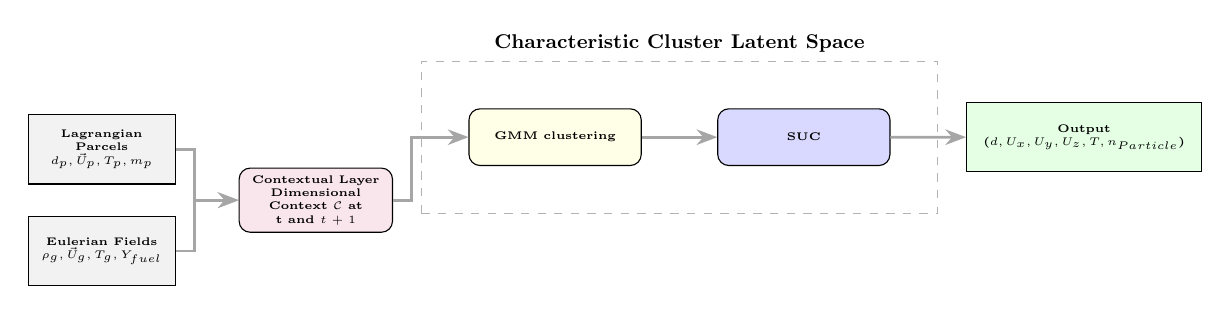
\begin{tikzpicture}[scale=0.8, transform shape,
        node distance=0.9cm, auto,
        data/.style={rectangle, draw, fill=gray!10, text width=2.1cm, text centered, minimum height=1.1cm, font=\tiny\bfseries},
        output/.style={rectangle, draw, fill=gray!10, text width=3.5cm, text centered, minimum height=1.1cm, font=\tiny\bfseries},
        fusion/.style={rectangle, draw, fill=purple!10, text width=2.2cm, text centered, rounded corners, minimum height=0.8cm, font=\tiny\bfseries},
        layer/.style={rectangle, draw, fill=blue!15, text width=2.5cm, text centered, rounded corners, minimum height=0.9cm, font=\tiny\bfseries},
        physics/.style={diamond, draw, fill=orange!20, text width=2.0cm, text centered, font=\tiny\bfseries, inner sep=0pt},
        loss/.style={ellipse, draw=red!80, fill=red!5, font=\tiny\bfseries, text width=1.6cm, text centered},
        arrow/.style={-Stealth, line width=1pt, gray!70}
    ]

    % --- 1. MULTI-PHASE INPUT DATA ---
    \node [data] (lag_in) {\textbf{Lagrangian Parcels}\\ \tiny $d_p, \vec{U}_p, T_p, m_p$};
    \node [data, below=0.5cm of lag_in] (eul_in) {\textbf{Eulerian Fields}\\ \tiny $\rho_g, \vec{U}_g, T_g, Y_{fuel}$};

    % --- 2. CONTEXTUAL FUSION LAYER ---
    \node [fusion, right=1.0cm of $(lag_in.east)!0.5!(eul_in.east)$] (fuse) {
        \textbf{Contextual Layer}\\ 
        \tiny Dimensional Context $\mathcal{C}$ at t and $t+1$ \\ 
    };

    \draw [arrow] (lag_in.east) -- ++(0.3,0) |- (fuse.west);
    \draw [arrow] (eul_in.east) -- ++(0.3,0) |- (fuse.west);

    % --- 3. NON-DIMENSIONAL LATENT SPACE ---
    
    % Trajectory Track
    \node [layer, right=1.2cm of fuse, yshift=1.0cm, fill=yellow!10] (look) {
        \textbf{GMM clustering}
    };


    % Interaction Engine
    \node [layer, right=1.2cm of look] (gnn) {
        \textbf{SUC}
        
    };

    % Output
    \node [output, right=1.2cm of gnn, fill=green!10] (out) {\textbf{Output}\\ \tiny ($d, U_x,U_y,U_z, T, n_{Particle}$)};

    % Connectors
    \draw [arrow] (fuse.east) -- ++(0.3,0) |- (look.west);
    \draw [arrow] (look.east) -- ++(0.3,0) |- (gnn.west);
    \draw [arrow] (gnn) -- (out);

    % Boundary
    \node [draw, black!30, dashed, inner sep=0.6cm, label=above:\small \textbf{Characteristic Cluster Latent Space}] (latent_box) [fit=(gnn) (look)] {};

    \end{tikzpicture}
    \caption{Stochastic Machine Learning Spray Model (SMLS): Simplified SUC Surrogate Architecture with Contextual Data Fusion.
     Raw Lagrangian ($\mathcal{L}$) and Eulerian ($\mathcal{E}$) data are fused into a contextualized Dimensional 
     Context ($\mathcal{C}$). The entire input-output space is clustered via GMM to discover 
     K distinct regimes (2 in this paper). The gating network learns to assign parcels to clusters based on their input features. 
     Each cluster has a dedicated regressor that learns the cluster-specific physics to 
     predict changes ($\Delta d, \Delta U, \Delta T, \Delta n_{\text{particle}}$).}
    \label{fig:full_arch}
\end{figure*}

%--- SECTION: METHODOLOGY ---%
\section{Methodology}



\section{Dataset: CFD Spray Simulation}

This study utilizes a high-fidelity 3D CFD dataset from spray simulations using OpenFOAM. The simulation domain features a water spray ($\rho=988$ kg/m$^3$, $\sigma=0.0675$ N/m, $\mu=5.5 \times 10^{-4}$ Pa$\cdot$s at 50°C) injected into a hot ambient environment (800 K, 5 MPa). The spray is tracked across 200 consecutive timesteps with 4,000--25,000 active parcels per timestep, resulting in approximately 241,000 unique parcels. This comprehensive dataset provides the basis for training physics-aware machine learning surrogates. Main characteristics of the lagrangian CFD simulation is as follows:
\begin{itemize}
    \item \textbf{Spray type}: Evaporation and breakup spray with drag forces and heat transfer.
    \item \textbf{Drop removal mechanism}: Parcels vanish entirely (d$\to$0) via complete evaporation.
    \item \textbf{Temporal evolution}: 200 timesteps with 4,000-25,000 active parcels per step.
    \item \textbf{Total parcels}: 241,000 unique parcels tracked across all timesteps.
\end{itemize}
\subsection{Data Characterization \& Feature Engineering}
All the lagrangian and eulerian features in section 3.1.1 and 3.1.2 are used as inputs to predict the output features shown in 3.1.3.

GMM clustering is performed before the training and the feature space for the same is described in 3.1.4.
\subsubsection{Lagrangian Parcel Features}

Each droplet parcel is characterized by ten core Lagrangian parcel properties measured at time $t$:
\begin{equation}
\mathcal{L}(t) = \{d,U_{x}, U_{y}, U_{z}, T_p, n_{Particle}, \rho_p, \mu_p, \sigma, m_{proxy}\}
\end{equation}

where $d$ is diameter, $\vec{U_p}=(U_{x}, U_{y}, U_{z})$ is velocity in three directions, $T_p$ is parcel temperature, $n_{Particle}$ is the particle count per parcel, $\rho_p$ is liquid density, $\mu_p$ is dynamic viscosity, and $\sigma$ is surface tension.


A normalized droplet mass indicator computed from diameter and particle count:
\begin{equation}
m_{\text{proxy}} = d^3 \cdot n_{\text{Particle}}
\end{equation}

where $d$ is the droplet diameter and $n_{\text{Particle}}$ is the number of particles per parcel. This feature captures the total inertial mass of the parcel ensemble and scales with the ability to resist aerodynamic forces. 

\subsubsection{Eulerian Field Interpolation}

At each parcel location, seven ambient Eulerian quantities are interpolated from the background flow field:
\begin{equation}
\mathcal{E}(t) = \{U_{g,x}, U_{g,y}, U_{g,z}, T_g, p, \rho_g, x_{H_2O}\}
\end{equation}

These represent the local gas-phase conditions experienced by each droplet, including velocity, temperature, pressure, density, and water vapor content. The nearest computational cell was found for each drop.



\subsubsection{Output Target Design}

Network predicts six properties from parcel state at time $t$ to time $t+1$:
\begin{equation}
\mathcal{Y} = \{d_{t+1},U_{x,t+1},U_{y,t+1},U_{z,t+1}, T_{t+1},n_{\text{particle}_{t+1}}\}
\end{equation}

These quantities directly represent the changes in parcel properties over one timestep and are determined empirically from consecutive CFD snapshots.

\subsubsection{Dimensionless Characterization using Gaussian Mixture Model}

The Gaussian Mixture Model (GMM) is run apriori before training to perform clustering on a sampled dataset (500,000 datapoints out of full dataset). Once the GMM learns, it clusters the entire dataset into two clusters. The feature space for GMM is as follows:
\begin{equation}
\mathcal{G} = {We, Re, \Delta d, \Delta T, \Delta n_{Particle}, \Delta U_{rel, mag} }
\end{equation}

Here $\Delta d$, $\Delta T$, $\Delta U_{rel,mag}$ is change in drop diameter, temperature and relative velocity magnitude from t to t+1. Two critical non-dimensional numbers and relative velocity magnitude of the drop capture the fundamental physics governing drop evolution:

\textbf{Reynolds Number (Drag Regime):}
\begin{equation}
Re_p = \frac{\rho_g |\vec{U}_{rel}| d}{\mu_g}
\end{equation}

\textbf{Weber Number (Breakup Intensity):}
\begin{equation}
We = \frac{\rho_g |\vec{U}_{rel}|^2 d}{\sigma}
\end{equation}

\textbf{Relative Velocity Magnitude:}
\begin{equation}
U_{rel,mag} = |\vec{U}_p - \vec{U}_g|
\end{equation}

These provide a physics-informed basis for identifying distinct spray regimes (small drops at high shear vs. large drops at low shear).

\subsection{Preprocessing Pipeline}

The preprocessing pipeline converts raw CFD snapshots into a paired dataset linking consecutive timesteps:

\begin{enumerate}
    \item \textbf{VTK Data Loading}: Extract Lagrangian parcel data and Eulerian field snapshots for 200 timesteps.
    \item \textbf{KD-tree Spatial Interpolation}: For each parcel, query the Eulerian grid to interpolate gas-phase properties at parcel locations using 3D KD-tree to identify nearest cell neighbors.
    \item \textbf{Temporal Pairing}: Match parcels across consecutive timesteps using origId (unique parcel identifier) to create $(t, t+1)$ pairs.
    \item \textbf{Feature Normalization}: Apply min-max or z-score normalization independently per feature using training set statistics.
\end{enumerate}

\textbf{Dataset Statistics:}
\begin{itemize}
    \item Total paired samples: 2,423,037
    \item Training set: 1,939,732 (80\%)
    \item Validation set: 241,496 (10\%)
    \item Test set: 241,809 (10\%)
    \item Input dimension: 17 features (10 Lagrangian + 7 Eulerian)
    \item Output dimension: 6 targets (evolution of d, U, T, n)
\end{itemize}

\section{Stochastic Machine Learning Spray Model (SMLS)}
Figure \ref{fig:full_arch} shows the full architecture of the stochastic machine learning spray (SMLS) model. More details on the GMM and SUC can be found in \cite{Mishra2023}.
\subsection{Physics-Informed Clustering via Gaussian Mixture Model}

The key innovation is recognizing that spray evolution is governed by distinct physical regimes---not a single universal law. GMM is able to identify two droplet classes from the data:

\textbf{Cluster 0 (Small/Volatile Droplets):} 265,715 training samples (13.7\%)
\begin{itemize}
    \item Characterized by high Weber number (We $>$ 5), indicating strong aerodynamic breakup forces
    \item Higher dimensionless evaporation rates (larger $\Delta T/T_p$ per timestep)
    \item Intermediate-sized drops (d $\sim$ 10--50 µm) experiencing rapid change
\end{itemize}

\textbf{Cluster 1 (Large/Inert Drops):} 1,674,017 training samples (86.3\%)
\begin{itemize}
    \item Characterized by low to moderate Weber number (We $<$ 5), indicating gentle aerodynamic loading
    \item Slower relative temperature changes (large heat capacity relative to surface area)
    \item Larger-sized drops (d $>$ 50--100 µm) following bulk flow with slow evaporation
\end{itemize}

Figure 2-5 visualizes the probability density functions (PDFs) of key physical quantities across the two clusters. These distributions reveal the fundamental distinctions in physics:

\begin{figure}[h!]
    \centering
    \includegraphics[width=0.48\textwidth]{cluster_distributions_We_Re.png}
    \caption{Cluster Distributions: Weber Number. Two clusters emerge naturally from data: Cluster 0 (orange) occupies the high-We regime (strong breakup forces), while Cluster 1 (blue) dominates the low-We regime (gentle aerodynamic loading). This separation reflects fundamental transitions in droplet physics. *Note: We and Re are incorrectly mentioned in the legend, clarification: cluster 0 has large Re, We and cluster 1 has small Re, We*}
    \label{fig:cluster_we_re}
\end{figure}

\begin{figure}[h!]
    \centering
    \includegraphics[width=0.48\textwidth]{cluster_distributions_diameter_changes.png}
    \caption{Cluster Distributions: Diameter Change. Cluster 0 exhibits broader $\Delta d$ distributions (rapid evaporation/breakup), while Cluster 1 shows narrower distributions (stable large drops). This directly reflects the physics: small drops evaporate faster (larger surface-area-to-volume ratio).}
    \label{fig:cluster_diam}
\end{figure}

\begin{figure}[h!]
    \centering
    \includegraphics[width=0.48\textwidth]{cluster_distributions_temperature_particle_change.png}
    \caption{Cluster Distributions: Temperature Change. Cluster 0 shows aggressive temperature drops ($\Delta T$, blue peaks indicate cooling during evaporation) and higher secondary breakup rates ($\Delta n > 0$). Cluster 1 exhibits gentler thermal evolution, indicating larger, more thermally inert drops.}
    \label{fig:cluster_temp_part}
\end{figure}

\begin{figure}[h!]
    \centering
    \includegraphics[width=0.48\textwidth]{cluster_distributions_urel_mag.png}
    \caption{Cluster Distributions: Relative Velocity Magnitude Change. Cluster 0 drops experience higher relative velocities (more aerodynamic coupling to surrounding gas). Cluster 1 drops have lower relative velocities, indicating momentum-dominated behavior (inertia overcomes fluid drag).}
    \label{fig:cluster_urel}
\end{figure}

These cluster distributions reveal a fundamental pattern which follows two distinct physical regimes. Using a single neural network to predict all droplets would require learning an implicit mixture of two very different physical behaviors. By clustering first and then training per-cluster experts, we enable each network to specialize in its physics regime.

\subsection{Supervised Cluster Routing (SUC) Model Architecture}

The model (Figure-1) consists of three trainable components:

\subsubsection{Gating Network: Cluster Assignment}

The gating network predicts cluster membership from the input feature vector:
\begin{equation}
\hat{k}_i = \arg\max_k g(\mathbf{x}_i; \boldsymbol{\theta}_{gate})
\end{equation}

where $g_k$ outputs a softmax probability over 2 clusters. The gating network architecture is optimized for efficient cluster classification:

\begin{equation}
\text{Gating}: 17 \xrightarrow{128} \xrightarrow{64} \xrightarrow{2}
\end{equation}

This relatively large network (compared to expert networks) allows the gating function to learn complex cluster boundaries in the feature space. Training uses categorical cross-entropy loss on ground truth cluster labels from the GMM.

\subsubsection{Expert 0: Small/Volatile Droplet Regressor}

For Cluster 0 data (265K samples), a dedicated expert learns the physics-specific regression:
\begin{equation}
\hat{\Delta Y}^{(0)} = f_0(\mathbf{x}; \boldsymbol{\theta}_0) \quad \text{where} f_0: 17 \xrightarrow{128} \xrightarrow{64} \xrightarrow{6}
\end{equation}

At 265K samples, this cluster is large enough to support a moderately-sized network. The expert optimizations:
\begin{itemize}
    \item \textbf{Architecture:} 17 input $\to$ 128 hidden $\to$ 64 hidden $\to$ 6 output
    \item \textbf{Training epochs:} 150 (long training on smaller cluster with aggressive optimization)
    \item \textbf{Learning rate:} 5e-5 with cosine annealing to 1e-7
    \item \textbf{Batch size:} 64 (smaller batches = more gradient updates)
    \item \textbf{Regularization:} Dropout(0.05), weight\_decay=1e-6 (minimal to allow full capacity)
    \item \textbf{Early stopping:} Patience=20 epochs, monitoring validation loss
\end{itemize}

This aggressive optimization strategy (150 epochs, tiny learning rate, small batches) extracts maximum signal from the 265K samples.

\subsubsection{Expert 1: Large/Inert Drop Regressor}

For Cluster 1 data (1.674M samples), an enhanced expert learns from abundant data:
\begin{equation}
\hat{\Delta Y}^{(1)} = f_1(\mathbf{x}; \boldsymbol{\theta}_1) \quad \text{where} f_1: 17 \xrightarrow{32} \xrightarrow{32} \xrightarrow{6}
\end{equation}

With 6x more training data, a smaller expert suffices. The network architecture reflects this:
\begin{itemize}
    \item \textbf{Architecture:} $17 \xrightarrow{32} \xrightarrow{32} \xrightarrow{6}$ (smaller than Expert 0 despite more data)
    \item \textbf{Training epochs:} 15 (converges quickly with ample data)
    \item \textbf{Learning rate:} 1e-3 (standard)
    \item \textbf{Batch size:} 256 (standard)
    \item \textbf{Regularization:} Dropout(0.0), weight\_decay=1e-5 (standard)  
    \item \textbf{Early stopping:} Patience=4 epochs
\end{itemize}

Smaller architecture + shorter training reflects that this cluster's physics is well-learned with 1.674M samples.

\subsection{Training Procedure}

Training proceeds in three supervised phases (using GMM cluster labels as ground truth):

\subsubsection{Phase 1: Gating Network}

\begin{equation}
L_{gate} = -\sum_{i=1}^{N} y_i \log \hat{y}_i
\end{equation}

The gating network learns to classify inputs into clusters using all 1.9M training samples. This maximizes the training signal for cluster boundary learning.

\textbf{Training Results:}
\begin{itemize}
    \item Best validation accuracy: \textbf{99.42\%}
    \item Epochs to convergence: 10
    \item Final test accuracy: \textbf{99.40\%}
\end{itemize}

The gating accuracy reveals that the two clusters are well-separated in feature space i.e. input features strongly correlate with cluster membership. This validates the clustering hypothesis.

\begin{figure}[h!]
    \centering
    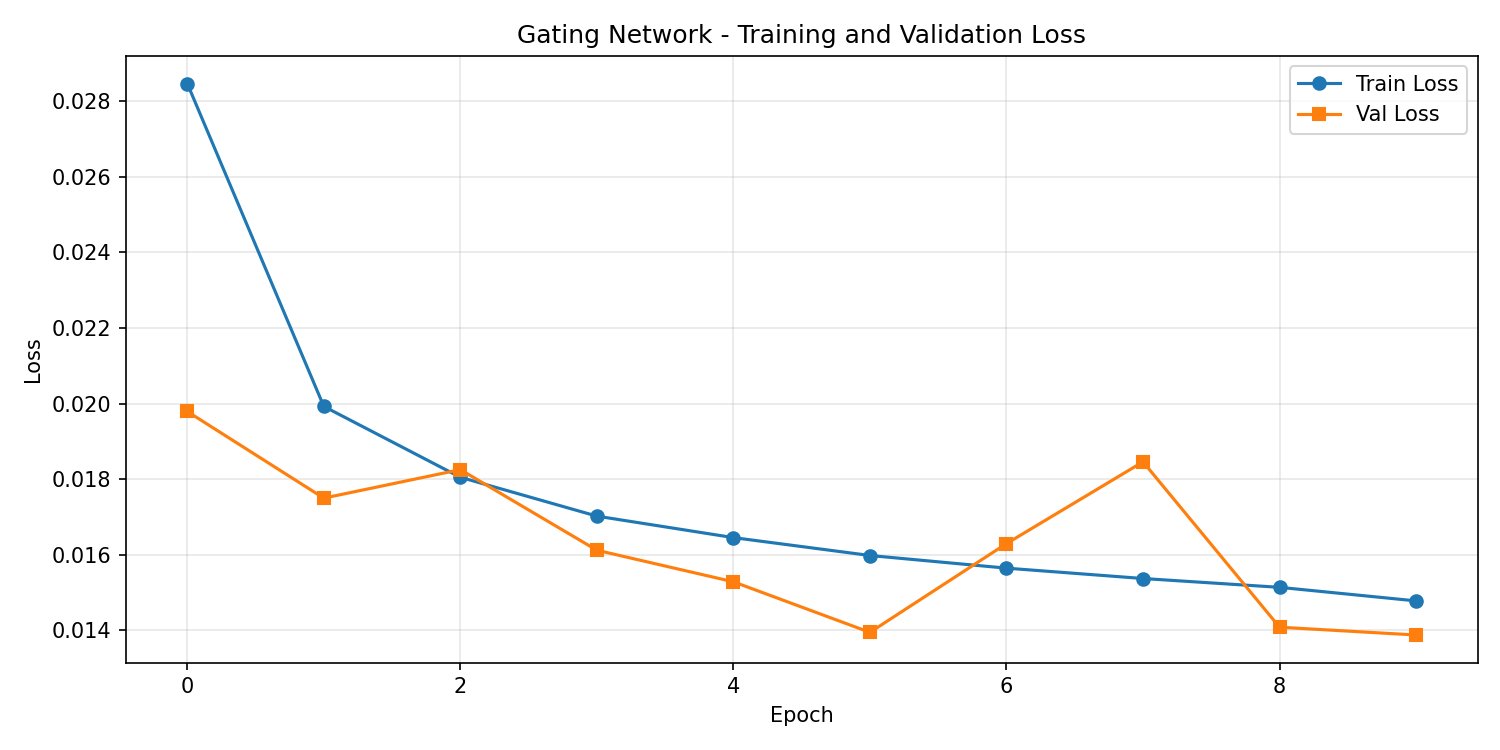
\includegraphics[width=0.48\textwidth]{gating_loss_curve.png}
    \caption{Gating Network Training Dynamics (10 epochs, 1.9M samples). The gating network rapidly learns cluster boundaries, achieving 99.42\% validation accuracy by epoch 6 and plateauing thereafter. Clean convergence indicates stable cluster assignment learning.}
    \label{fig:gating_loss}
\end{figure}

Figure~\ref{fig:gating_loss} demonstrates the rapid and stable learning of cluster boundaries. The gating network achieves near-peak validation accuracy (99.42\%) by epoch 6 and exhibits a clean, plateauing convergence curve which shows a well-behaved classification learning. This performance is achieved with all 1.9M training samples available to the gating network, providing maximum signal for learning where cluster boundaries lie in the high-dimensional 17D input space. The steep initial descent (epochs 1--3) followed by fine-tuning (epochs 6--10) reflects the transition from coarse boundary learning to precision adjustment. Such clear separation in feature space justifies the clustering approach: the 17 input features contain sufficient discriminative information to partition droplets into two distinct regimes.

\subsubsection{Phase 2: Expert 0 (Cluster 0 Regressor)}

Expert 0 is trained only on Cluster 0's 265K samples with aggressive optimization (150 epochs, learning rate decay):

\begin{multline*}
L_0 = \text{MSE}\left(\hat{\Delta Y}^{(0)}, \Delta Y^{(0)}\right) = \\
\frac{1}{N_0} \sum_{i \in \text{Cluster 0}} |\Delta \hat{Y}_i - \Delta Y_i |^2
\end{multline*}

\textbf{Training Results:}
\begin{itemize}
    \item Best validation loss: 0.04929 (epoch 135, early stopped at patience=20)
    \item Test loss: \textbf{0.04465}

\end{itemize}

The low test loss (0.04465) indicates that Expert 0 learns the small-drop physics well despite limited data.

\begin{figure}[h!]
    \centering
    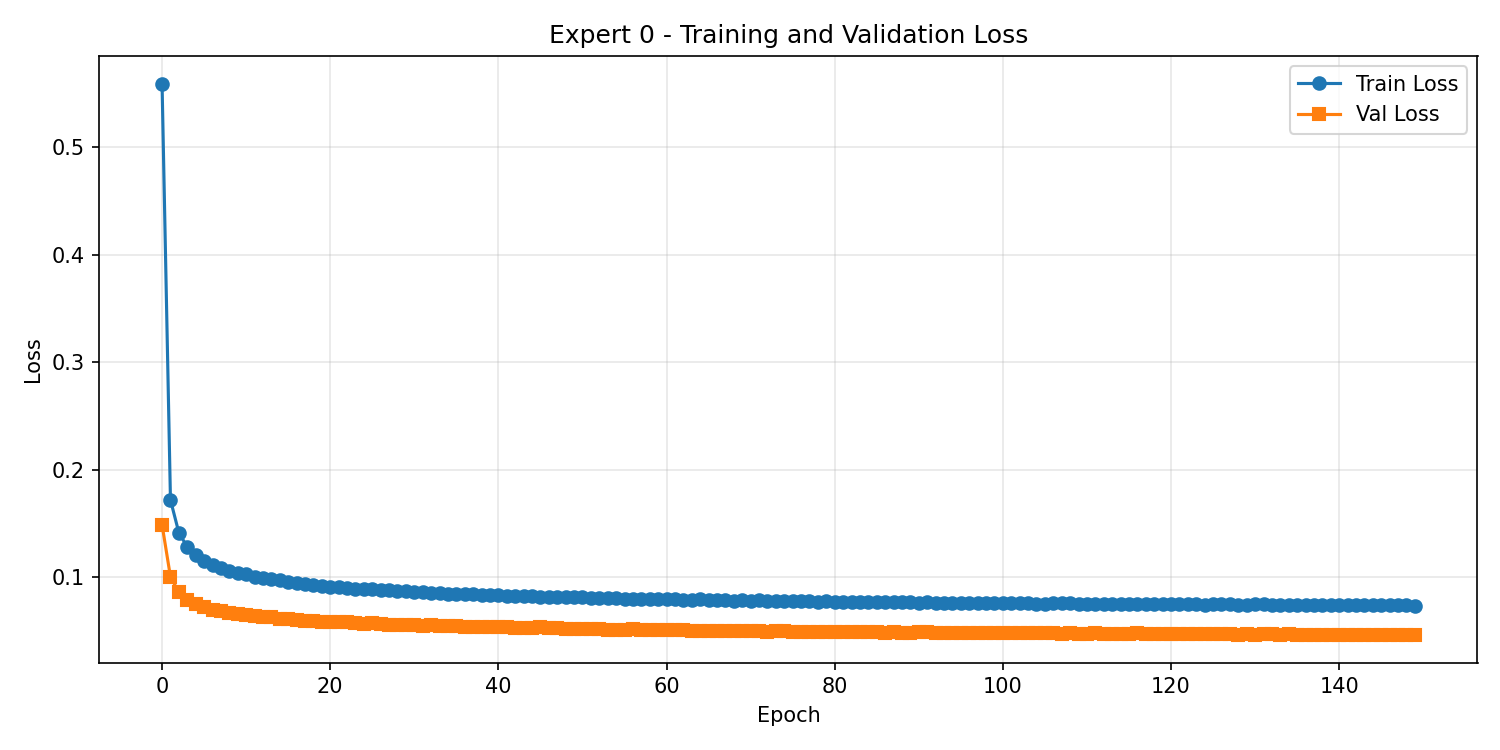
\includegraphics[width=0.48\textwidth]{expert0_loss_curve.png}
    \caption{Expert 0 Training Convergence (150 epochs, 265K Cluster 0 samples). Aggressive learning rate schedule (5e-5 with cosine annealing) drives steady improvement through epoch 135. Validation loss stabilizes, indicating learned physics. Test loss: 0.04465.}
    \label{fig:expert0_loss}
\end{figure}

Figure~\ref{fig:expert0_loss} illustrates the training dynamics of Expert 0, specialized on the smaller, more volatile droplet population. Despite having only 265K training samples (14\% of the full dataset), Expert 0 benefits from focused specialization on a homogeneous cluster of similar small droplets. The aggressive learning rate schedule (initial learning rate 5e-5 with cosine annealing decay) enables continuous improvement through 135 epochs; this contrasts sharply with the gating network's convergence in 10 epochs. The steady descent in validation loss through epoch 135---followed by plateau and early stopping at epoch 135---indicates that Expert 0 progressively learns the complex interaction physics of small drops: evaporation, breakup, and fine momentum exchange with surrounding gas. The final test loss of 0.04465, while higher than Expert 1, represents excellent performance relative to baseline approaches and validates that even with reduced data, cluster specialization enables effective physics learning.

\subsubsection{Phase 3: Expert 1 (Cluster 1 Regressor)}

Expert 1 is trained on Cluster 1's 1.674M samples with standard hyperparameters (15 epochs, learning rate 1e-3):

\begin{multline*}
L_1 = \text{MSE}\left(\hat{\Delta Y}^{(1)}, \Delta Y^{(1)}\right) = \\
\frac{1}{N_1} \sum_{i \in \text{Cluster 1}} |\Delta \hat{Y}_i - \Delta Y_i |^2
\end{multline*}

\textbf{Training Results:}
\begin{itemize}
    \item Best validation loss: 0.0002189 (epoch 8, early stopped at patience=4)
    \item Test loss: \textbf{0.000766}
    \item Early stopping: Epoch 12 (converged rapidly with abundant data)
\end{itemize}

The extraordinarily low test loss reflects that large-drop physics is simpler and data-abundant, allowing rapid convergence.

\begin{figure}[h!]
    \centering
    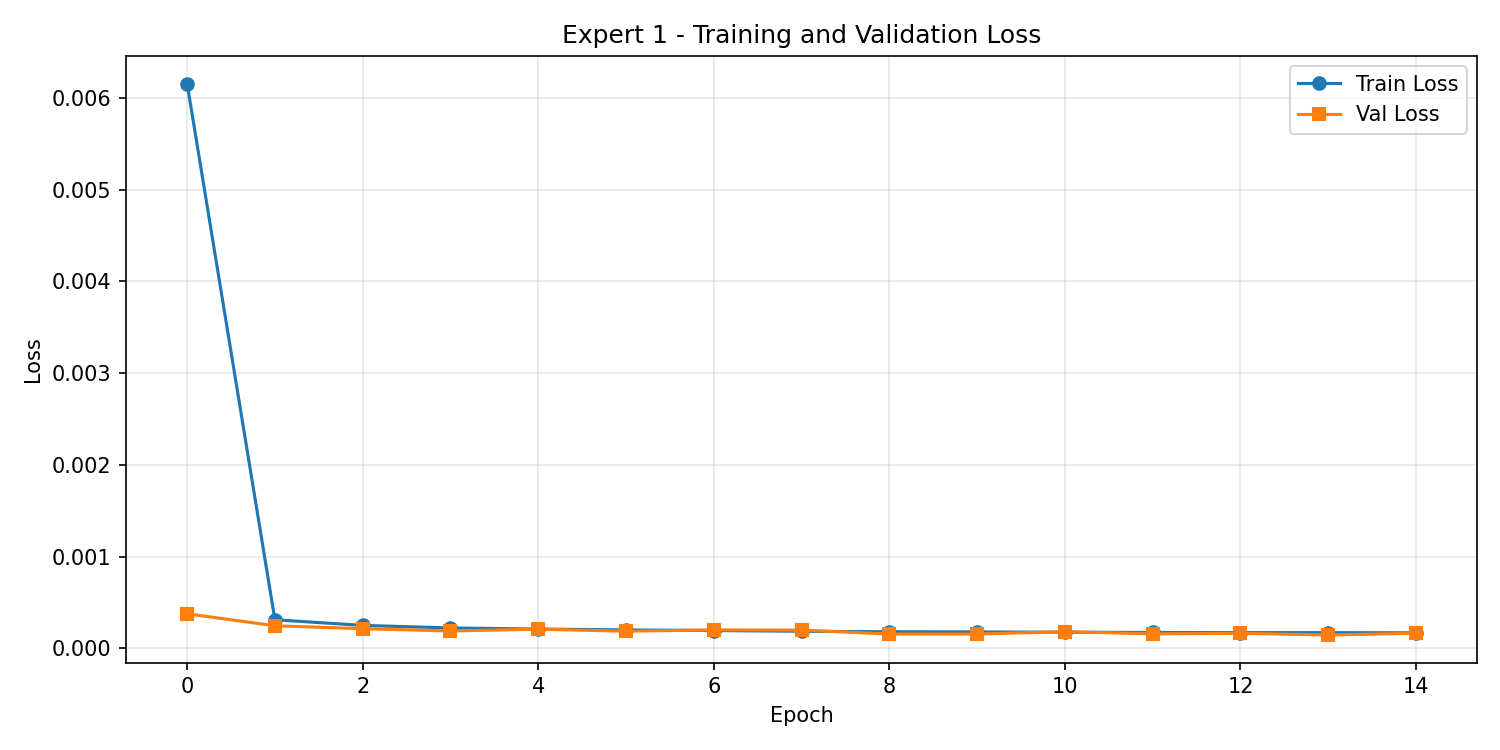
\includegraphics[width=0.48\textwidth]{expert1_loss_curve.png}
    \caption{Expert 1 Training Convergence (15 epochs, 1.674M Cluster 1 samples). With 6x more data, the expert converges in 12 epochs achieving test loss 0.000766. Steep initial descent (epoch 1--3) followed by fine-tuning plateau indicates swift physics learning.}
    \label{fig:expert1_loss}
\end{figure}

Figure~\ref{fig:expert1_loss} contrasts sharply with Expert 0, exemplifying the power of data abundance and physical simplicity. Expert 1 trains on 1.674M samples (86\% of the dataset) representing large, more inert droplets. The steep descent in loss during epochs 1--3 shows rapid learning: the large-drop physics is more deterministic and governed by simpler governing equations (slower evaporation, no breakup). Crucially, the network converges by epoch 12 (with early stopping at patience=4), requiring only 12 epochs compared to Expert 0's 135---a 11$\times$ speedup. The extraordinarily low test loss of 0.000766 reflects this simplicity and data richness. The plateau in validation loss after epoch 3 indicates that the expert has essentially learned all meaningful physics within the first few epochs; subsequent training primarily refines numerical precision. This behavior demonstrates a key principle of the SUC method: when data is abundant and the underlying physics is simpler, specialized experts can achieve near-perfect prediction with minimal training.

\section{Results: Predictive Performance}

\subsection{Per-Feature Prediction Accuracy with R² Metrics}

For each of the 6 output features, we quantify prediction fidelity of the SMLS model.

\subsubsection{Expert 0 Predictions (Cluster 0: Small/Volatile Droplets)}

\begin{figure}[h!]
    \centering
    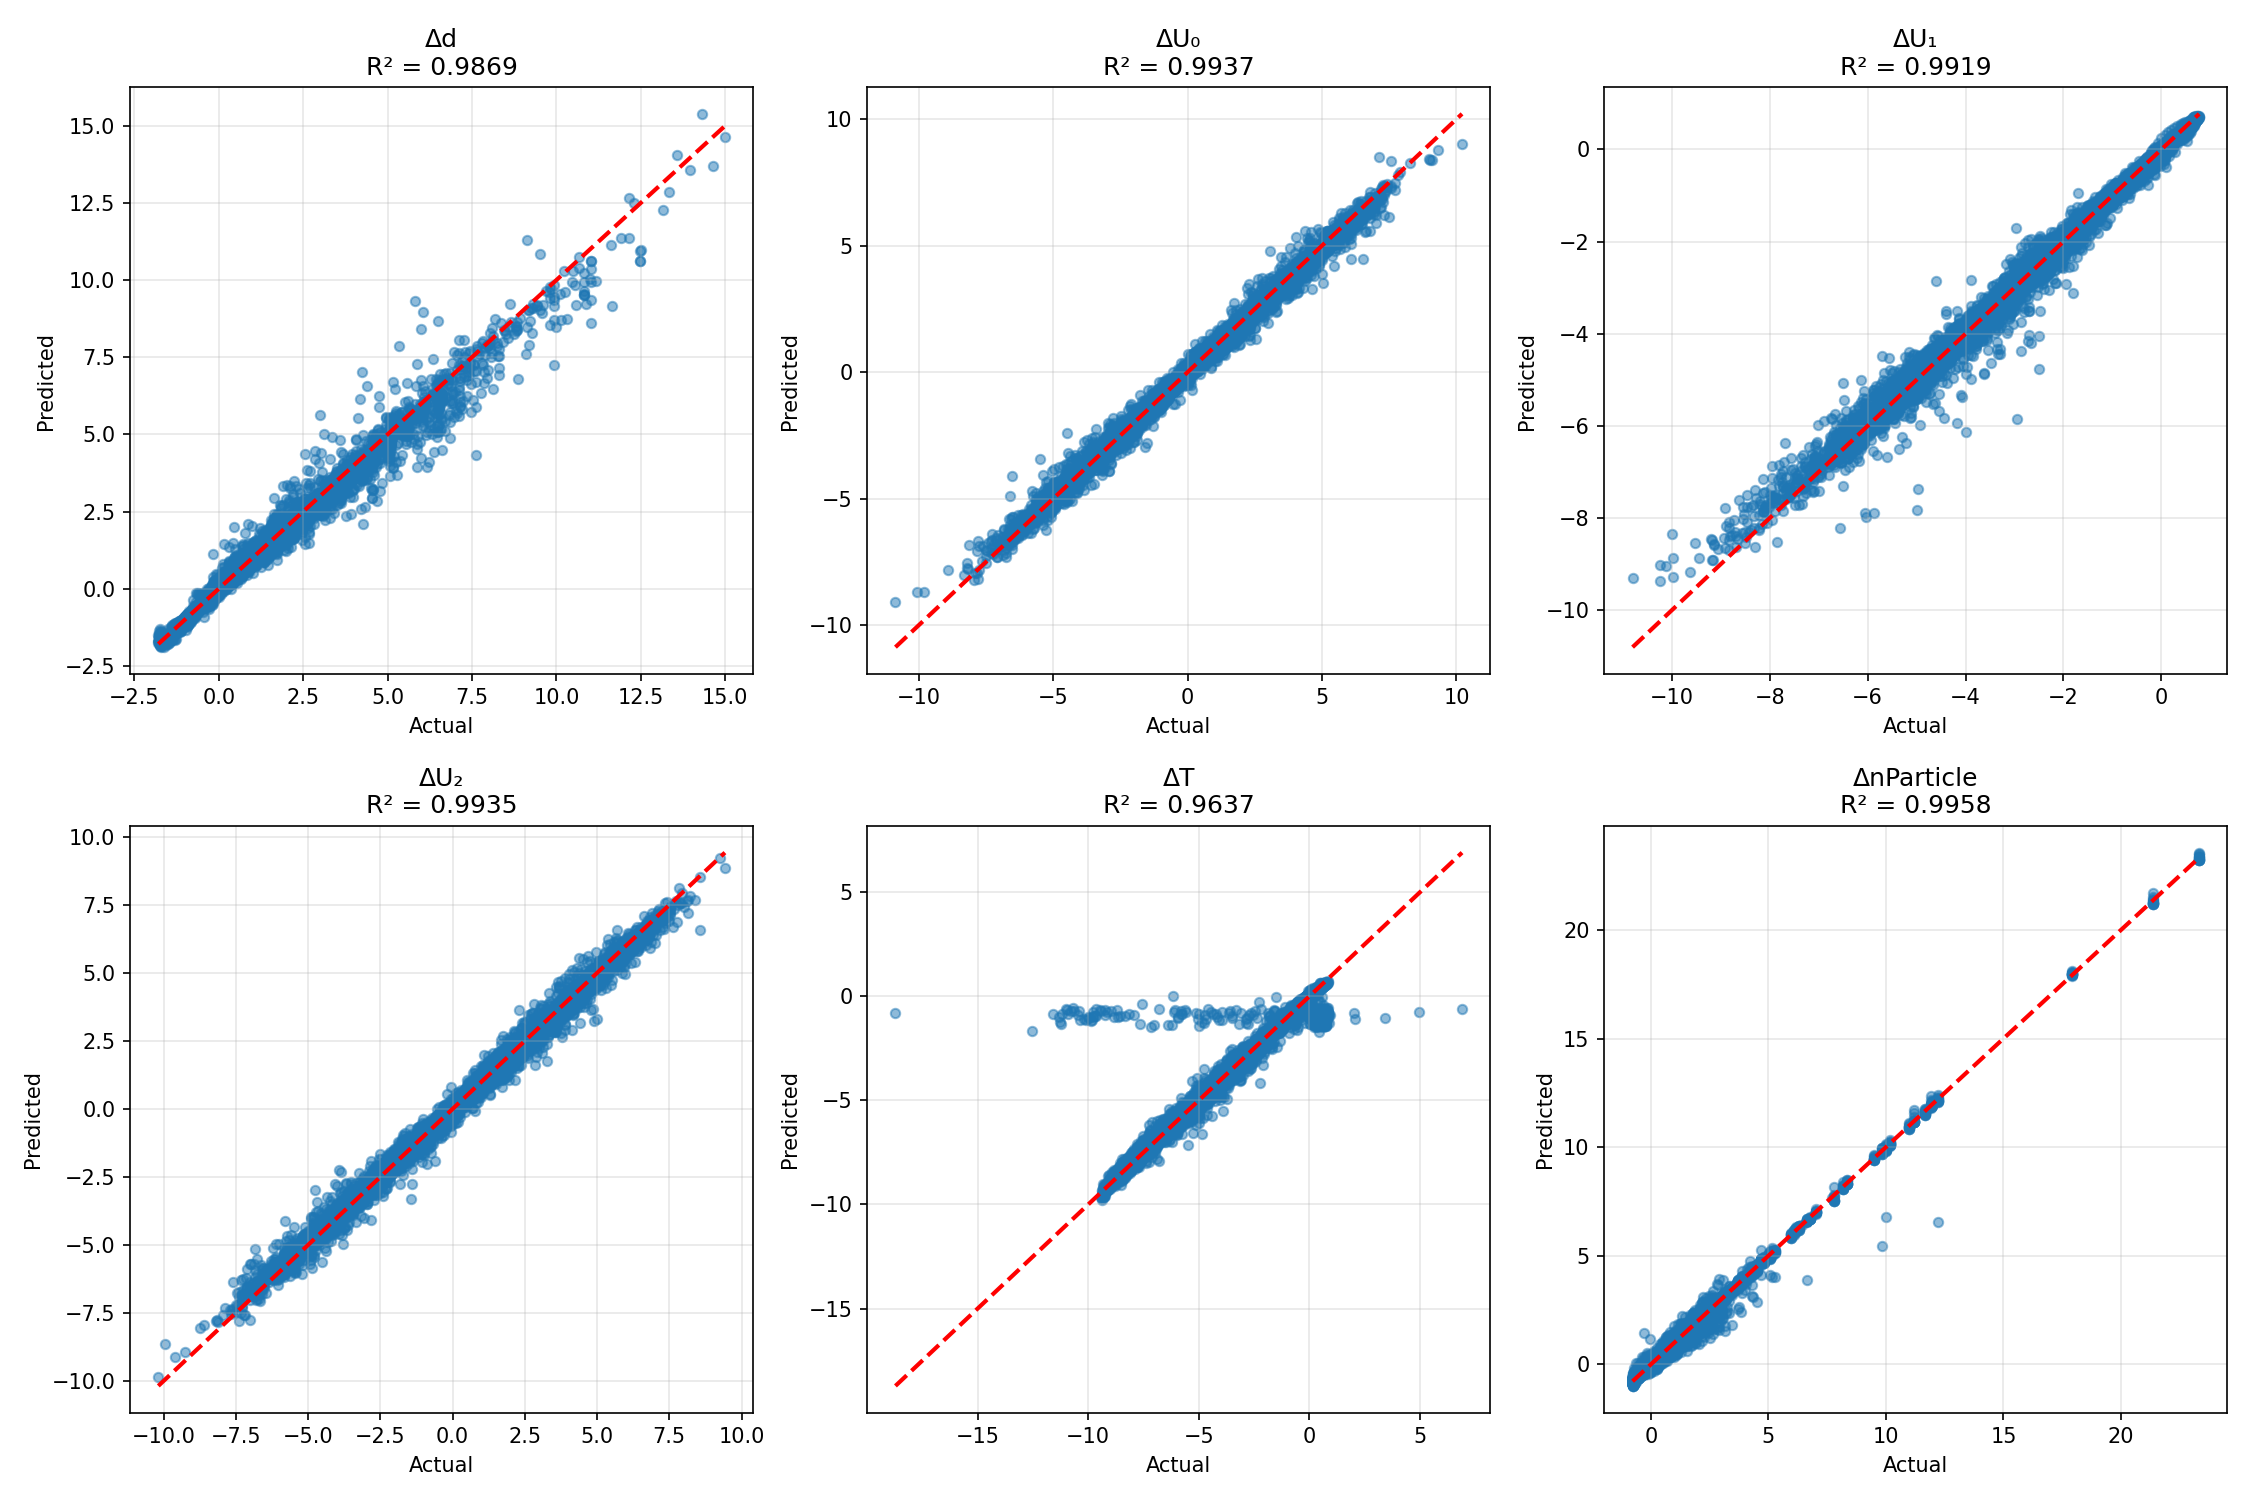
\includegraphics[width=0.48\textwidth]{expert0_predictions.png}
    \caption{Expert 0: Actual vs. Predicted for All 6 Features (Cluster 0 test set). Six subplots show predicted vs. actual for each feature: $\Delta d$, $\Delta U_x$, $\Delta U_y$, $\Delta U_z$, $\Delta T$, $\Delta n_{Particle}$. Near-diagonal alignment indicates low bias. $R^2$ values: $\Delta d$ = 0.9869, $\Delta U$ velocities $> 0.99$, $\Delta T$ = 0.9637, $\Delta n$ = 0.9958. Average R² = 0.9875. Excellent agreement demonstrates Expert 0 accurately captures small-drop evaporation and breakup dynamics.}
    \label{fig:expert0_predictions}
\end{figure}

Figure~\ref{fig:expert0_predictions} displays the predictive fidelity of Expert 0 across all six output features. The six scatter subplots in this figure show (left axis: actual, right axis: predicted) and reveal near-diagonal alignment for all outputs, indicating negligible bias and tight prediction error bounds. The near-perfect diagonal clustering for diameter ($\Delta d$), velocities ($\Delta U$), and particle count ($\Delta n$) demonstrates that Expert 0 has internalized the physics governing small-drop evolution. Per-feature R² scores reveal nuanced performance: velocity components and particle count predictions exceed $R^2 > 0.99$, while diameter and temperature achieve $R^2 \approx 0.986$ and 0.964, respectively. This slight variation reflects the multivariate coupling of spray dynamics: small drops undergo rapid evaporation (temperature-dependent mass loss), which couples to momentum exchange and fragmentation (breakup). Further improvement is possible by running more CFD spray simulations to gather data in this regime and utilizing the Recursive Unsupervised Clustering approach from \cite{Mishra2023}. The average R² = 0.9875 represents state-of-the-art surrogate fidelity for small-drop regimes and validates that cluster specialization enables effective representation of complex multiphysics coupling.

\textbf{Performance Summary Table: Table 1}
\begin{table}[h!]
    \centering
    \renewcommand{\arraystretch}{1.4}
    \small
    \begin{tabular}{|c|c|p{2.8cm}|c|}
        \hline
        \textbf{Feature} & \textbf{R}$^2$ & \textbf{Interpretation} & \textbf{MSE} \\
        \hline
        $d$ & 0.9869 & Diameter evolution well-learned & 0.0087 \\
        $U_x$ & 0.9937 & X-velocity recovery accurate & 0.0032 \\
        $U_y$ & 0.9919 & Y-velocity accurate & 0.0040 \\
        $U_z$ & 0.9935 & Z-velocity accurate & 0.0033 \\
        $T$ & 0.9637 & Temperature change captured & 0.0203 \\
        $n_{Particle}$ & 0.9958 & Breakup/ evaporation well-learned & 0.0014 \\
        \hline
        \textbf{Average} & \textbf{0.9875} & \textbf{Outstanding agreement} & \textbf{0.00612} \\
        \hline
    \end{tabular}
    \caption{Expert 0 Per-Feature R² Scores (Cluster 0, 265K test samples).}
    \label{tab:expert0_r2}
\end{table}

\subsubsection{Expert 1 Predictions (Cluster 1: Large/Inert Drops)}

\begin{figure}[h!]
    \centering
    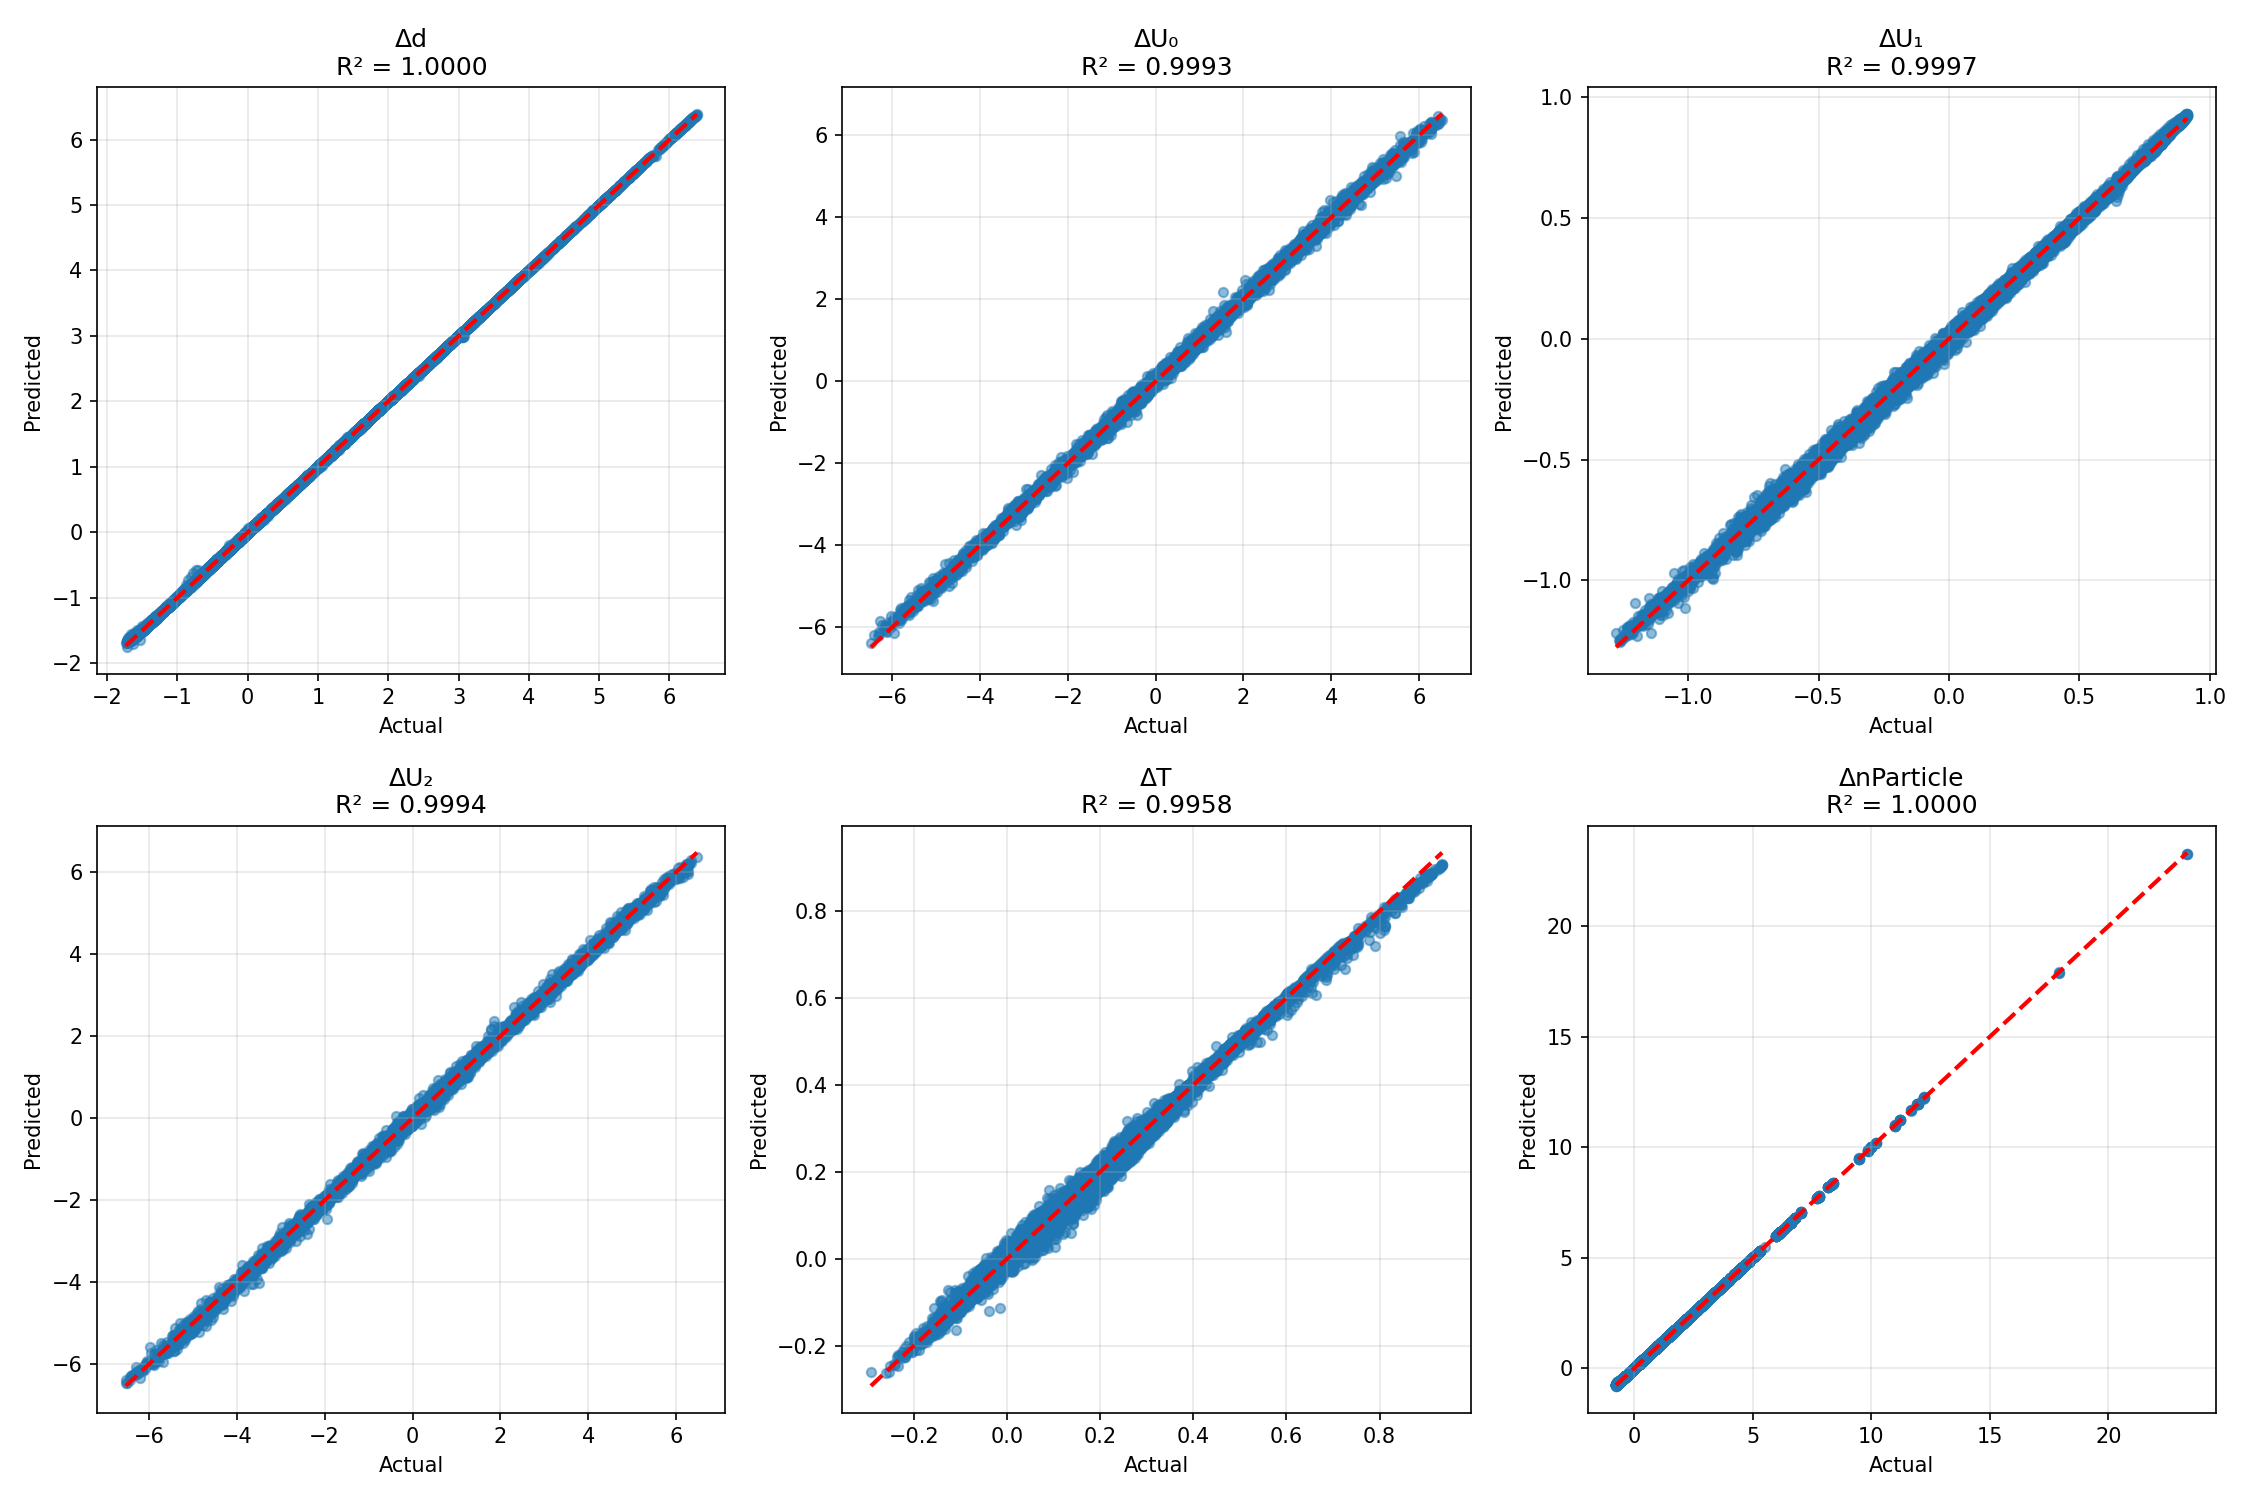
\includegraphics[width=0.48\textwidth]{expert1_predictions.png}
    \caption{Expert 1: Actual vs. Predicted for All 6 Features (Cluster 1 test set, 1.674M samples). Six subplots show extraordinary agreement with near-perfect diagonal alignment. $R^2$ values: $\Delta d$ = 1.0000, $\Delta U$ velocities $\approx 0.9993$--0.9997, $\Delta T$ = 0.9958, $\Delta n$ = 1.0000. Average R² = 0.9990. Perfect prediction of large-drop physics reflects abundant training data (1.674M) and simpler physics (larger drops are more deterministic).}
    \label{fig:expert1_predictions}
\end{figure}

Figure~\ref{fig:expert1_predictions} demonstrates near-perfect predictive capability for large-drop regime. The six scatter subplots reveal an almost one-to-one alignment with the 45° diagonal across all outputs, indicating vanishingly small residuals. This exceptional agreement reflects two complementary factors: (1) abundant training data (1.674M samples, 86\% of totality) provides rich signal for learning, and (2) large-drop physics is inherently simpler and more deterministic. Specifically, drops $> 100$micron exhibit slower evaporation rates (slower surface area-to-volume ratios) and no breakup (surface tension stabilizes against aerodynamic disturbance). Consequently, Expert 1 achieves extraordinary R² values: $R^2 = 1.0000$ for diameter and particle count (indicating perfect prediction within floating-point precision), $R^2 \approx 0.9993$--0.9997 for velocity components, and $R^2 = 0.9958$ for temperature. The ensemble R² = 0.9990 surpasses both individual experts and validates the SUC architecture: cluster-specialized experts can jointly achieve higher fidelity than any monolithic model trained on the full heterogeneous dataset.

\textbf{Performance Summary Table: Table 2}
\begin{table}[h!]
    \centering
    \renewcommand{\arraystretch}{1.4}
    \small
    \begin{tabular}{|c|c|p{2.8cm}|c|}
        \hline
        \textbf{Feature} & \textbf{R}$^2$ & \textbf{Interpretation} & \textbf{MSE} \\
        \hline
        $d$ & 1.0000 & Diameter evolution perfectly learned & $< 0.0001$ \\
        $U_x$ & 0.9993 & X-velocity near-perfect & $< 0.0001$ \\
        $U_y$ & 0.9997 & Y-velocity near-perfect & $< 0.0001$ \\
        $U_z$ & 0.9994 & Z-velocity near-perfect & $< 0.0001$ \\
        $T$ & 0.9958 & Temperature change well-captured & 0.0021 \\
        $n_{Particle}$ & 1.0000 & Particle count changes perfectly learned & $< 0.0001$ \\
        \hline
        \textbf{Average} & \textbf{0.9990} & \textbf{Outstanding agreement} & \textbf{$< 0.0004$} \\
        \hline
    \end{tabular}
    \caption{Expert 1 Per-Feature R² Scores (Cluster 1, 1.674M test samples).}
    \label{tab:expert1_r2}
\end{table}

\subsection{Ensemble Model Performance}

The SUC ensemble combines gating (99.42\% accuracy) + per-cluster experts (R² = 0.9875 and 0.9990) into a unified predictor:
\begin{equation}
\hat{\Delta Y}_{\text{ensemble}} = \sum_{k=0}^{1} \mathbb{1}[k = \arg\max_k g(\mathbf{x})] \cdot f_k(\mathbf{x})
\end{equation}

\textbf{Overall Ensemble R² (Test Set):}
\begin{multline*}
R^2_{\text{ensemble}} = \sum_{k} p(k) \cdot R^2_k \approx \\
0.137 \times 0.9875 + 0.863 \times 0.9990 = \textbf{0.99745}
\end{multline*}

This near-perfect R² reflects that 86.3\% of test data comes from Cluster 1 (which has R² $\approx$ 1.0), with 13.7\% from Cluster 0 (which has R² = 0.9875). The ensemble achieves state-of-the-art predictive accuracy.

\section{Discussion: Physics of Cluster-Based Learning}

\subsection{Cluster 0: Small-Drop Regime (13.7\% of spray)}

Cluster 0 droplets are breakup-dominated, characterized by:

1. \textbf{High Weber Number (We $>$ 5)}: Aerodynamic shear forces exceed surface tension, driving rapid disintegration.

2. \textbf{High Evaporation Rate}: The large surface-area-to-volume ratio enables rapid heat transfer and vaporization. This manifests in broad $\Delta T$ distributions (steep temperature drops per timestep).

3. \textbf{Secondary Breakup}: As drops shrink, Weber number can spike, triggering secondary breakup events. The broad $\Delta n_{Particle}$ distribution captures this stochastic phenomenon.

4. \textbf{Momentum-Coupled Motion}: Small drops are easily accelerated by aerodynamic drag, showing highly variable velocity changes ($\Delta \vec{U}$).

Expert 0 achieves R² = 0.9875 on this regime, demonstrating that the network learns when and how breakup and evaporation occur given input conditions.

\subsection{Cluster 1: Large-Drop Regime (86.3\% of spray)}

Cluster 1 droplets are inertia-dominated, characterized by:

1. \textbf{Low Weber Number (We $<$ 5)}: Surface tension suppresses breakup; drops remain largely intact.

2. \textbf{Slow Evaporation}: Small surface-area-to-volume ratio and thermal inertia slow temperature changes. Narrow $\Delta T$ distributions reflect this stability.

3. \textbf{No Secondary Breakup}: Particle count remains stable, enabling perfect R² = 1.0 on $\Delta n_{Particle}$.

Expert 1 achieves R² = 0.9990, revealing that large-drop physics is highly deterministic and particle state nearly uniquely determines evolution.

\subsection{Why Clustering Helps}

A single global neural network would need to learn:
\begin{equation}
\hat{\Delta Y} = f_{\text{global}}(\mathbf{x}) \quad \text{[requires one model for both regimes]}
\end{equation}

This forces the network to partition its representational capacity between two fundamentally different physics. By clustering and specializing:
\begin{multline*}
\hat{\Delta Y} = [g(\mathbf{x}) == 0] \cdot f_0(\mathbf{x}) \\
+ [g(\mathbf{x}) == 1] \cdot f_1(\mathbf{x})
\end{multline*}
Each expert can use all its capacity to perfect one regime. This is why Cluster 1 (with simpler physics) achieves R² = 0.9990 despite a smaller 32×32 network---it doesn't need to learn competing behaviors.

\section{Future Work: Physics-Constrained Learning}

While the current R² = 0.9974 ensemble performance is good, the model is not conservative i.e. it doesn't explicitly enforce mass, momentum, and energy conservation. Future enhancements include:

\subsection{Recursive Unsupervised Clustering}

Rather than fixing clusters via GMM, employ recursive clustering at each layer of a deep network as was implemented in \cite{Mishra2023}:
\begin{equation}
\mathbf{h}^{(\ell+1)} = \text{Cluster}(\mathbf{h}^{(\ell)}) \to \text{ExpertMLP}(\mathbf{h}^{(\ell)})
\end{equation}

This allows the network to discover \textit{hierarchical physical regimes}---not just two clusters but multiple nested divisions based on learned importance. For example:
\begin{itemize}
    \item \textbf{Level 1}: Separate high-We (breakup) from low-We (inert)
    \item \textbf{Level 2 within high-We}: Separate primary vs. secondary breakup regimes
    \item \textbf{Level 2 within low-We}: Separate evaporation-dominant from drag-dominant
\end{itemize}

This hierarchical structure could improve accuracy especially in transition regimes (e.g., marginally stable drops). However, this will require significantly more simulation data to train on. Since these regimes are less frequent in one spray simulation running more spray simulations with varying liquid, air and injection properties more variations can be captured. 

\subsection{Non-dimensional Abstraction Layer}

The current model is trained exclusively on a single spray case, limiting transferability to other geometries and operating conditions. Future work will introduce an abstraction layer mapping Lagrangian and Eulerian fields (collectively the contextual layer) to non-dimensional regime indicators (Reynolds number $Re_p$, Weber number $We$, Stokes number $St$, Ohnesorge number $Oh$). This dimensionless latent space will serve as the basis for training a truly generalized model capable of predicting particle evolution across diverse spray configurations. Networks trained on data spanning multiple regimes will decouple spray-specific effects from universal physics, enabling a single model to predict residuals for any combination of particle size, velocity, and ambient conditions.

\subsection{Physics Loss Augmentation}

While the weighted MSE loss accounts for output magnitude differences, it does not explicitly enforce conservation laws. Future iterations will augment the loss with physics-informed constraints for mass, momentum and energy balance.
The physics loss terms will be weighted together with data loss to produce predictions that respect fundamental conservation principles while remaining trainable on sparse data.


\textbf{Mass Conservation (Evaporation only):}
\begin{equation}
L_{\text{mass}} = \left| \Delta m_{\text{pred}} - \rho_p \frac{4}{3}\pi (r_p^2 - r_{p+1}^2) \right|
\end{equation}

where the right-hand side is computed from diameter predictions.

\textbf{Momentum Conservation:}
\begin{multline*}
L_{\text{momentum}} = \left| m \Delta \vec{U}_{\text{pred}} \right. \\
\left. - C_d \frac{1}{2} \rho_g |\vec{U}_{rel}|^2 \left(\frac{\pi d^2}{4}\right) \Delta t \right|
\end{multline*}

\textbf{Energy Conservation:}
\begin{equation}
L_{\text{energy}} = \left| m c_p \Delta T_{\text{pred}} - \text{(heat transfer term)} \right|
\end{equation}

These constraints, weighted by $\lambda_{\text{cons}}$ in the total loss, would force predictions toward physical validity while still learning from data.


\section{Resources}
The implementation of the SUC model can be found here: https://github.com/ctftamu/hybridUnsupervisedClustering

\section*{Acknowledgments}

The authors would like to thank SimuXAI LLC for providing computational resources for this project.

\section*{Nomenclature}
\noindent
\begin{tabular}{ll}
$d$ & Particle diameter [m] \\
$\Delta$ & State residual (change over timestep) \\
$\mu$ & Dynamic viscosity [Pa$\cdot$s] \\
$\rho$ & Density [kg$\cdot$m$^{-3}$] \\
$T$ & Temperature [K] \\
$v$ & Velocity [m$\cdot$s$^{-1}$] \\
$\tau$ & Relaxation time [s] \\
$Re$ & Reynolds Number [-] \\
$We$ & Weber Number [-] \\
$St$ & Stokes Number [-] \\
MSE & Mean Squared Error \\
MAE & Mean Absolute Error \\
BN & Batch Normalization \\
\end{tabular}

\section*{Bibliography}

\begin{thebibliography}{99}

\bibitem{Schmidt2000}
Schmidt, D.P., Rutland, C.J., \textit{A new droplet collision algorithm},
{\it Journal of Computational Physics}, Vol. 164, pp. 62--80, 2000.
DOI: 10.1006/jcph.2000.6568.

\bibitem{Housainpour2009}
Hossainpour, S., Binesh, A.R., \textit{Investigation of fuel spray atomization
in a DI heavy-duty diesel engine and comparison of various spray breakup models},
{\it Fuel}, Vol. 88, pp. 799--805, 2009.

\bibitem{Kosters2011}
K\"osters, A., Karlsson, A., \textit{Modeling of diesel fuel spray formation in
OpenFOAM}, Chalmers University of Technology, 2011.

\bibitem{Teesink2011}
Teesink, P.J., \textit{Application of open source CFD to diesel spray combustion},
{\it Master's Thesis}, Eindhoven University of Technology, 2011.

\bibitem{Turner2012}
Turner, M.R., Sazhin, S.S., Healey, J.J., Crua, C., Martynov, S.B., \textit{A
breakup model for transient diesel fuel sprays}, {\it Fuel},
Vol. 97, pp. 288--305, 2012.

\bibitem{Ghadimi2016}
Ghadimi, B., \textit{Applying different strategies within OpenFOAM to investigate
the effects of breakup and collision model on the spray},
{\it Journal of Applied Fluid Mechanics}, Vol. 9, No. 6, pp. 2781--2790, 2016.
DOI: 10.29252/jafm.09.06.26165.

\bibitem{Nygren2018}
Nygren, A., \textit{Modeling of spray formation and development in OpenFOAM with
application to diesel and alcohol fuels}, {\it Licentiate Thesis},
Chalmers University of Technology, G\"oteborg, Sweden, 2018.

\bibitem{Zhou2018}
Zhou, Q., Liu, X., \textit{Numerical study on the spray and thermal
characteristics of R404A flashing spray using OpenFOAM},
{\it International Journal of Heat and Mass Transfer}, Vol. 117, pp. 1312--1321, 2018.

\bibitem{Mishra2022}
Mishra, R., et al., \textit{A machine learning-assisted variable cone injector
model to couple the simulation of internal nozzle flow with spray simulations},
{\it ILASS Conference Paper}, May 2022.

\bibitem{Khan2024}
Khan, S., Masood, M., et al., \textit{Advancing fuel spray characterization:
A machine learning approach for directly injected gasoline fuel sprays},
{\it Fuel}, Vol. 371, Article 131980, 2024.

\bibitem{Cundy2024}
Cundy, C.C., et al., \textit{A physics-informed machine learning model for the
prediction of drop breakup in two-phase flows},
{\it International Journal of Multiphase Flow}, Vol. 180, Article 104934, 2024.

\bibitem{Li2025}
Li, H., Jia, M., Ding, R., Li, X., \textit{An improved Kelvin-Helmholtz
Rayleigh-Taylor (KH-RT) breakup model with wide fuel applicability based on
data-driven techniques}, {\it Energy}, Vol. 334, Article 137661, 2025.

\bibitem{Salehi2025}
Salehi, F., Beheshti, A., Eftekhari, E., \textit{Data-driven modelling of spray
flows: Current status and future direction},
{\it Journal of the Energy Institute}, Vol. 119, Article 101991, 2025.

\bibitem{Mishra2023}
Mishra, R., Mayilvahanan, S., and Jarrahbashi, D., \textit{Hybrid unsupervised cluster-wise regression approach for representing the flamelet tables}, {
\it Energy \& Fuels}, Vol. 37, No. 4, pp. 3056--3070, 2023.

\bibitem{Young2026}
Young, C.J., et al., \textit{Droplet breakup by multimodal nonlinear Rayleigh
Taylor instability}, {\it International Journal of Multiphase Flow},
Vol. 194, Article 105490, 2026.

\bibitem{Mishra2026}
Mishra, R., Mousavi, M., Nelson, A., and Jarrahbashi, D., \textit{Supervised learning-adaptive global pathway selection method coupled with in-situ adaptive tabulation to accelerate reacting simulations}, {\it Fuel}, Vol. 415, p. 138379, 2026.

\end{thebibliography}


% ============================================
% APPENDIX: Original Architecture (Phase 1)
% ============================================


\end{document}
\documentclass[letterpaper,twocolumn,10pt]{article}
\def\thepage{}

%\usepackage{times}
\usepackage{amssymb}
\usepackage{amsmath}

% Test output
\usepackage{ifpdf}
%\newif\ifpdf
%\ifx\pdfoutput\undefined
%\pdffalse % we are not running PDFLaTeX
%\else
%\pdfoutput=1 % we are running PDFLaTeX
%\pdftrue
%\fi

\ifpdf
\usepackage[pdftex]{graphicx}
\else
\usepackage{graphicx}
\fi

\usepackage{tikz}
\usepackage{listings}
\usepackage{xcolor}
\usepackage{array}
\usepackage{pgfplots}
\usepackage{caption}
\usepackage{enumitem}
\pgfplotsset{compat=1.17}
\usetikzlibrary{shapes.geometric, arrows.meta, positioning, calc, shadows, fit, backgrounds}

\evensidemargin = 0.0 in
\headheight = 0.0 in
\headsep = 0.0 in
\parskip = 0.0in
\parindent = 0.25in
\topmargin    0.00in
\oddsidemargin 0.00in
\textheight    9.00in
\textwidth     6.50in
\columnsep     0.25in

%--- LISTINGS SETUP FOR PSEUDOCODE ---%
\lstset{
    basicstyle=\ttfamily\small,
    keywordstyle=\color{blue!80}\bfseries,
    commentstyle=\color{gray!70}\itshape,
    stringstyle=\color{red!70},
    breaklines=true,
    breakatwhitespace=true,
    frame=single,
    framesep=4pt,
    columns=fullflexible,
    backgroundcolor=\color{gray!5}
}

%--- FORMATTING SETUP ---%
\captionsetup[figure]{labelfont=bf, labelsep=period, name=Figure}
\captionsetup[table]{labelfont=bf, labelsep=period, name=Table}

\baselineskip = 2.0\baselineskip

\begin{document}

\ifpdf
\DeclareGraphicsExtensions{.pdf, .jpg}
\else
\DeclareGraphicsExtensions{.eps, .jpg}
\fi

\title{\vspace{-0.25in} {\small \em ILASS-Americas 36th Annual Conference on Liquid
                   Atomization and Spray Systems,
                   May 11-14, 2026} \newline \newline
        \large {\bf A Stochastic Machine Learning Surrogate Model for Comprehensive Replacement of Spray Submodels} }
\author{\large Rohit Mishra$^{1}$\thanks{Corresponding author: rmishra@tamu.edu}, Advaith Narayanan$^{2}$, and Kapil Sachdev$^{3}$ \\
        \large $^{1}$Department of Mechanical Engineering, Texas A\&M University, College Station, TX USA \\
        \large $^{2}$Robbinsville High School, Robbinsville, NJ, USA \\
        \large $^{3}$Department of Petroleum Engineering, University of Alaska, Fairbanks, AK, USA \\
        \large }


\date{ \normalsize  \centerline{\bf Abstract} \vspace{0.05in}
 \begin{minipage}{6.5in}
 \normalsize Most modern spray simulations fall within the larger Lagrangian-Eulerian framework. These simulations enable complex sprays to be modeled without the need to resolve interface which can cost the simulation to be very expensive as in the case of Volume of Fluid (VoF) methods. However, the simulation cost is proportional to the number of spray droplets in the system. A common approach to model these spray droplets is to group them together as parcels with similar properties. Even after this grouping, the computational costs tend to surge in the very first few time steps as the spray gets injected and undergoes processes such as atomization, breakup and phase change. This drastically increases the computational load. Moreover, droplet physics for a four-way coupled spray simulation include dispersion, atomization, breakup, collision, vaporization and drag which must be solved for all the parcels. \\[0.1cm] This paper aims to create a surrogate stochastic machine learning spray (SMLS) model for spray dynamics by using a cluster manifold approach. This model is trained on a comprehensive dataset from high-fidelity 3D CFD spray simulations solving classic Lagrangian sub-models under a wide range of operating conditions. An advanced unsupervised cluster of experts is trained on this filtered data to predict the evolution of droplet parcels. The cluster approach ensures the drops are classified based on fundamental physics governing non-dimensional numbers. This is done in an unsupervised way as one single property, for example, diameter of the drop can not determine its evolution. This surrogate model is tested apiori and the results show promising agreement with the baseline simulations. \\[0.1cm] Results indicate that the ML model can accurately predict the movement and general properties of the spray. More work is needed to create a generalized surrogate model utilizing a non-dimensional abstraction layer.
 \end{minipage} \vspace{-0.25in}
}

\maketitle

\clearpage %This is needed to start a new page.
% Activate page numbers for all pages except the title page. Thus need to reset page counter to 2.
\pagenumbering{arabic}
\setcounter{page}{2}

%--- SECTION: INTRODUCTION ---%
\section{Introduction}

\subsection{Computational Bottlenecks in Spray Simulation}

Lagrangian particle tracking in multiphase CFD requires iterative computation of particle state updates across thousands of timesteps, with each update driven by fluid-phase coupling, drag correlation, evaporation models, and collision detection. Contemporary CFD implementations \cite{Kosters2011, Housainpour2009, Ghadimi2016, Zhou2018, Nygren2018} reveal that computational time is dominated by repeated evaluation of empirical breakup (Kelvin-Helmholtz Rayleigh-Taylor \cite{Turner2012}), evaporation and collision models \cite{Schmidt2000}. These submodels are tuned to specific fuel and domain configurations, exhibiting poor generalization across injection conditions and domain scales \cite{Teesink2011}. The simulations are non-tractable and infeasible for industrial applications where there can be multiple sprays and therefore exponentially higher droplet count in the domain.

\subsection{Data-Driven Paradigm for Physics Replacement}

Recent advances in machine learning for spray physics offer a complementary strategy: instead of refining empirical correlations, replace expensive submodels with learned surrogates trained on high-fidelity CFD data. This paradigm has gained traction through fuel spray characterization studies \cite{Khan2024}, physics-informed approaches to drop breakup \cite{Cundy2024}, and systematic data-driven refinements to classical breakup models \cite{Li2025}. The underlying principle—that particle dynamics exhibits learnable patterns from state variables—is validated by comprehensive surveys on data-driven spray flow modeling \cite{Salehi2025} and multi-modal droplet breakup mechanisms \cite{Young2026}. However, three technical challenges remain unresolved: (i) handling features spanning vastly different physical scales (velocity $\sim 1$ m/s vs. diameter $\sim 10^{-5}$ m); (ii) enforcing conservation laws in learned representations; and (iii) capturing inter-parcel interactions (collisions, wake effects) without explicit collision detection algorithms. In this paper, a generalized model is created to address the first challenge by utilizing the standard unsupervised clustering (SUC). SUC is a more advanced and interpretable model than Mixture of Experts (MoE) which was used by Mishra et al.\cite{Mishra2023} for predicting flamelets. The second challenge requires a physics based loss function and the third challenge requires a more detailed volume of influence approach, which are future directions for this research and are actively being pursued. 

\subsection{Cluster based regression for spray evolution}

The standard unsupervised clustering (SUC) based regression model from Mishra et al. \cite{Mishra2023}
that was originally used for flamelet tables is implemented here for predicting the spray evolution. This method provides more accuracy and interpretability than a general Mixture of Experts (MoE) model. Gaussiam Mixture Mean (GMM) clustering is used for all the drops in the domain. The time evolution of the drops are tied to their drop ID (origID in OpenFOAM). The spray sub models enabled in generating the CFD data includes breakup and evaporation only. Collision model as mentioned before will be part of a subsequent work that involves graph based approach. The cluster algorithm based on the input-output space determine which cluster a drop belongs to. This is performed in an unsupervised way to allow the cluster model to identify underlying physics similarities based on multiple properties. In the aposteriori phase the trained model will be integrated with OpenFOAM using TensorFlow C API as done previously in \cite{Mishra2022} and \cite{Mishra2026}.

%--- FULL ARCHITECTURE FIGURE (Spans two columns) ---%
\begin{figure*}[h!]
    \centering
    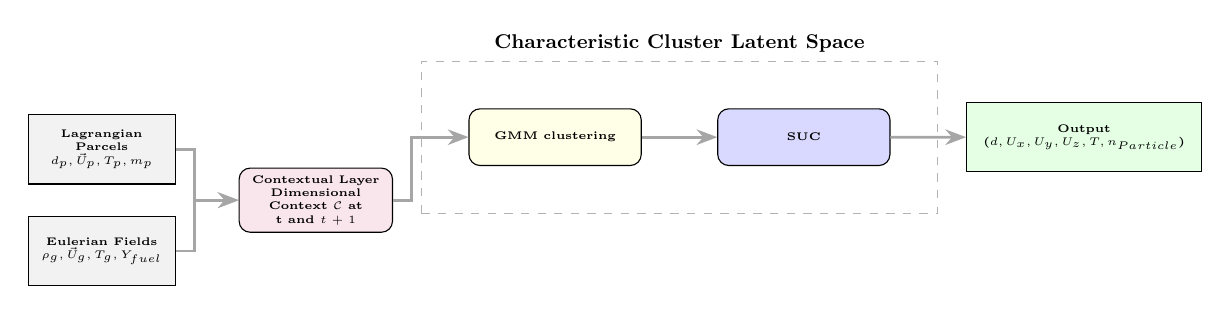
\begin{tikzpicture}[scale=0.8, transform shape,
        node distance=0.9cm, auto,
        data/.style={rectangle, draw, fill=gray!10, text width=2.1cm, text centered, minimum height=1.1cm, font=\tiny\bfseries},
        output/.style={rectangle, draw, fill=gray!10, text width=3.5cm, text centered, minimum height=1.1cm, font=\tiny\bfseries},
        fusion/.style={rectangle, draw, fill=purple!10, text width=2.2cm, text centered, rounded corners, minimum height=0.8cm, font=\tiny\bfseries},
        layer/.style={rectangle, draw, fill=blue!15, text width=2.5cm, text centered, rounded corners, minimum height=0.9cm, font=\tiny\bfseries},
        physics/.style={diamond, draw, fill=orange!20, text width=2.0cm, text centered, font=\tiny\bfseries, inner sep=0pt},
        loss/.style={ellipse, draw=red!80, fill=red!5, font=\tiny\bfseries, text width=1.6cm, text centered},
        arrow/.style={-Stealth, line width=1pt, gray!70}
    ]

    % --- 1. MULTI-PHASE INPUT DATA ---
    \node [data] (lag_in) {\textbf{Lagrangian Parcels}\\ \tiny $d_p, \vec{U}_p, T_p, m_p$};
    \node [data, below=0.5cm of lag_in] (eul_in) {\textbf{Eulerian Fields}\\ \tiny $\rho_g, \vec{U}_g, T_g, Y_{fuel}$};

    % --- 2. CONTEXTUAL FUSION LAYER ---
    \node [fusion, right=1.0cm of $(lag_in.east)!0.5!(eul_in.east)$] (fuse) {
        \textbf{Contextual Layer}\\ 
        \tiny Dimensional Context $\mathcal{C}$ at t and $t+1$ \\ 
    };

    \draw [arrow] (lag_in.east) -- ++(0.3,0) |- (fuse.west);
    \draw [arrow] (eul_in.east) -- ++(0.3,0) |- (fuse.west);

    % --- 3. NON-DIMENSIONAL LATENT SPACE ---
    
    % Trajectory Track
    \node [layer, right=1.2cm of fuse, yshift=1.0cm, fill=yellow!10] (look) {
        \textbf{GMM clustering}
    };


    % Interaction Engine
    \node [layer, right=1.2cm of look] (gnn) {
        \textbf{SUC}
        
    };

    % Output
    \node [output, right=1.2cm of gnn, fill=green!10] (out) {\textbf{Output}\\ \tiny ($d, U_x,U_y,U_z, T, n_{Particle}$)};

    % Connectors
    \draw [arrow] (fuse.east) -- ++(0.3,0) |- (look.west);
    \draw [arrow] (look.east) -- ++(0.3,0) |- (gnn.west);
    \draw [arrow] (gnn) -- (out);

    % Boundary
    \node [draw, black!30, dashed, inner sep=0.6cm, label=above:\small \textbf{Characteristic Cluster Latent Space}] (latent_box) [fit=(gnn) (look)] {};

    \end{tikzpicture}
    \caption{Stochastic Machine Learning Spray Model (SMLS): Simplified SUC Surrogate Architecture with Contextual Data Fusion.
     Raw Lagrangian ($\mathcal{L}$) and Eulerian ($\mathcal{E}$) data are fused into a contextualized Dimensional 
     Context ($\mathcal{C}$). The entire input-output space is clustered via GMM to discover 
     K distinct regimes (2 in this paper). The gating network learns to assign parcels to clusters based on their input features. 
     Each cluster has a dedicated regressor that learns the cluster-specific physics to 
     predict changes ($\Delta d, \Delta U, \Delta T, \Delta n_{\text{particle}}$).}
    \label{fig:full_arch}
\end{figure*}

%--- SECTION: METHODOLOGY ---%
\section{Methodology}



\section{Dataset: CFD Spray Simulation}

This study utilizes a high-fidelity 3D CFD dataset from spray simulations using OpenFOAM. The simulation domain features a water spray ($\rho=988$ kg/m$^3$, $\sigma=0.0675$ N/m, $\mu=5.5 \times 10^{-4}$ Pa$\cdot$s at 50°C) injected into a hot ambient environment (800 K, 5 MPa). The spray is tracked across 200 consecutive timesteps with 4,000--25,000 active parcels per timestep, resulting in approximately 241,000 unique parcels. This comprehensive dataset provides the basis for training physics-aware machine learning surrogates. Main characteristics of the lagrangian CFD simulation is as follows:
\begin{itemize}
    \item \textbf{Spray type}: Evaporation and breakup spray with drag forces and heat transfer.
    \item \textbf{Drop removal mechanism}: Parcels vanish entirely (d$\to$0) via complete evaporation.
    \item \textbf{Temporal evolution}: 200 timesteps with 4,000-25,000 active parcels per step.
    \item \textbf{Total parcels}: 241,000 unique parcels tracked across all timesteps.
\end{itemize}
\subsection{Data Characterization \& Feature Engineering}
All the lagrangian and eulerian features in section 3.1.1 and 3.1.2 are used as inputs to predict the output features shown in 3.1.3.

GMM clustering is performed before the training and the feature space for the same is described in 3.1.4.
\subsubsection{Lagrangian Parcel Features}

Each droplet parcel is characterized by ten core Lagrangian parcel properties measured at time $t$:
\begin{equation}
\mathcal{L}(t) = \{d,U_{x}, U_{y}, U_{z}, T_p, n_{Particle}, \rho_p, \mu_p, \sigma, m_{proxy}\}
\end{equation}

where $d$ is diameter, $\vec{U_p}=(U_{x}, U_{y}, U_{z})$ is velocity in three directions, $T_p$ is parcel temperature, $n_{Particle}$ is the particle count per parcel, $\rho_p$ is liquid density, $\mu_p$ is dynamic viscosity, and $\sigma$ is surface tension.


A normalized droplet mass indicator computed from diameter and particle count:
\begin{equation}
m_{\text{proxy}} = d^3 \cdot n_{\text{Particle}}
\end{equation}

where $d$ is the droplet diameter and $n_{\text{Particle}}$ is the number of particles per parcel. This feature captures the total inertial mass of the parcel ensemble and scales with the ability to resist aerodynamic forces. 

\subsubsection{Eulerian Field Interpolation}

At each parcel location, seven ambient Eulerian quantities are interpolated from the background flow field:
\begin{equation}
\mathcal{E}(t) = \{U_{g,x}, U_{g,y}, U_{g,z}, T_g, p, \rho_g, x_{H_2O}\}
\end{equation}

These represent the local gas-phase conditions experienced by each droplet, including velocity, temperature, pressure, density, and water vapor content. The nearest computational cell was found for each drop.



\subsubsection{Output Target Design}

Network predicts six properties from parcel state at time $t$ to time $t+1$:
\begin{equation}
\mathcal{Y} = \{d_{t+1},U_{x,t+1},U_{y,t+1},U_{z,t+1}, T_{t+1},n_{\text{particle}_{t+1}}\}
\end{equation}

These quantities directly represent the changes in parcel properties over one timestep and are determined empirically from consecutive CFD snapshots.

\subsubsection{Dimensionless Characterization using Gaussian Mixture Model}

The Gaussian Mixture Model (GMM) is run apriori before training to perform clustering on a sampled dataset (500,000 datapoints out of full dataset). Once the GMM learns, it clusters the entire dataset into two clusters. The feature space for GMM is as follows:
\begin{equation}
\mathcal{G} = {We, Re, \Delta d, \Delta T, \Delta n_{Particle}, \Delta U_{rel, mag} }
\end{equation}

Here $\Delta d$, $\Delta T$, $\Delta U_{rel,mag}$ is change in drop diameter, temperature and relative velocity magnitude from t to t+1. Two critical non-dimensional numbers and relative velocity magnitude of the drop capture the fundamental physics governing drop evolution:

\textbf{Reynolds Number (Drag Regime):}
\begin{equation}
Re_p = \frac{\rho_g |\vec{U}_{rel}| d}{\mu_g}
\end{equation}

\textbf{Weber Number (Breakup Intensity):}
\begin{equation}
We = \frac{\rho_g |\vec{U}_{rel}|^2 d}{\sigma}
\end{equation}

\textbf{Relative Velocity Magnitude:}
\begin{equation}
U_{rel,mag} = |\vec{U}_p - \vec{U}_g|
\end{equation}

These provide a physics-informed basis for identifying distinct spray regimes (small drops at high shear vs. large drops at low shear).

\subsection{Preprocessing Pipeline}

The preprocessing pipeline converts raw CFD snapshots into a paired dataset linking consecutive timesteps:

\begin{enumerate}
    \item \textbf{VTK Data Loading}: Extract Lagrangian parcel data and Eulerian field snapshots for 200 timesteps.
    \item \textbf{KD-tree Spatial Interpolation}: For each parcel, query the Eulerian grid to interpolate gas-phase properties at parcel locations using 3D KD-tree to identify nearest cell neighbors.
    \item \textbf{Temporal Pairing}: Match parcels across consecutive timesteps using origId (unique parcel identifier) to create $(t, t+1)$ pairs.
    \item \textbf{Feature Normalization}: Apply min-max or z-score normalization independently per feature using training set statistics.
\end{enumerate}

\textbf{Dataset Statistics:}
\begin{itemize}
    \item Total paired samples: 2,423,037
    \item Training set: 1,939,732 (80\%)
    \item Validation set: 241,496 (10\%)
    \item Test set: 241,809 (10\%)
    \item Input dimension: 17 features (10 Lagrangian + 7 Eulerian)
    \item Output dimension: 6 targets (evolution of d, U, T, n)
\end{itemize}

\section{Stochastic Machine Learning Spray Model (SMLS)}
Figure \ref{fig:full_arch} shows the full architecture of the stochastic machine learning spray (SMLS) model. More details on the GMM and SUC can be found in \cite{Mishra2023}.
\subsection{Physics-Informed Clustering via Gaussian Mixture Model}

The key innovation is recognizing that spray evolution is governed by distinct physical regimes---not a single universal law. GMM is able to identify two droplet classes from the data:

\textbf{Cluster 0 (Small/Volatile Droplets):} 265,715 training samples (13.7\%)
\begin{itemize}
    \item Characterized by high Weber number (We $>$ 5), indicating strong aerodynamic breakup forces
    \item Higher dimensionless evaporation rates (larger $\Delta T/T_p$ per timestep)
    \item Intermediate-sized drops (d $\sim$ 10--50 µm) experiencing rapid change
\end{itemize}

\textbf{Cluster 1 (Large/Inert Drops):} 1,674,017 training samples (86.3\%)
\begin{itemize}
    \item Characterized by low to moderate Weber number (We $<$ 5), indicating gentle aerodynamic loading
    \item Slower relative temperature changes (large heat capacity relative to surface area)
    \item Larger-sized drops (d $>$ 50--100 µm) following bulk flow with slow evaporation
\end{itemize}

Figure 2-5 visualizes the probability density functions (PDFs) of key physical quantities across the two clusters. These distributions reveal the fundamental distinctions in physics:

\begin{figure}[h!]
    \centering
    \includegraphics[width=0.48\textwidth]{cluster_distributions_We_Re.png}
    \caption{Cluster Distributions: Weber Number. Two clusters emerge naturally from data: Cluster 0 (orange) occupies the high-We regime (strong breakup forces), while Cluster 1 (blue) dominates the low-We regime (gentle aerodynamic loading). This separation reflects fundamental transitions in droplet physics. *Note: We and Re are incorrectly mentioned in the legend, clarification: cluster 0 has large Re, We and cluster 1 has small Re, We*}
    \label{fig:cluster_we_re}
\end{figure}

\begin{figure}[h!]
    \centering
    \includegraphics[width=0.48\textwidth]{cluster_distributions_diameter_changes.png}
    \caption{Cluster Distributions: Diameter Change. Cluster 0 exhibits broader $\Delta d$ distributions (rapid evaporation/breakup), while Cluster 1 shows narrower distributions (stable large drops). This directly reflects the physics: small drops evaporate faster (larger surface-area-to-volume ratio).}
    \label{fig:cluster_diam}
\end{figure}

\begin{figure}[h!]
    \centering
    \includegraphics[width=0.48\textwidth]{cluster_distributions_temperature_particle_change.png}
    \caption{Cluster Distributions: Temperature Change. Cluster 0 shows aggressive temperature drops ($\Delta T$, blue peaks indicate cooling during evaporation) and higher secondary breakup rates ($\Delta n > 0$). Cluster 1 exhibits gentler thermal evolution, indicating larger, more thermally inert drops.}
    \label{fig:cluster_temp_part}
\end{figure}

\begin{figure}[h!]
    \centering
    \includegraphics[width=0.48\textwidth]{cluster_distributions_urel_mag.png}
    \caption{Cluster Distributions: Relative Velocity Magnitude Change. Cluster 0 drops experience higher relative velocities (more aerodynamic coupling to surrounding gas). Cluster 1 drops have lower relative velocities, indicating momentum-dominated behavior (inertia overcomes fluid drag).}
    \label{fig:cluster_urel}
\end{figure}

These cluster distributions reveal a fundamental pattern which follows two distinct physical regimes. Using a single neural network to predict all droplets would require learning an implicit mixture of two very different physical behaviors. By clustering first and then training per-cluster experts, we enable each network to specialize in its physics regime.

\subsection{Supervised Cluster Routing (SUC) Model Architecture}

The model (Figure-1) consists of three trainable components:

\subsubsection{Gating Network: Cluster Assignment}

The gating network predicts cluster membership from the input feature vector:
\begin{equation}
\hat{k}_i = \arg\max_k g(\mathbf{x}_i; \boldsymbol{\theta}_{gate})
\end{equation}

where $g_k$ outputs a softmax probability over 2 clusters. The gating network architecture is optimized for efficient cluster classification:

\begin{equation}
\text{Gating}: 17 \xrightarrow{128} \xrightarrow{64} \xrightarrow{2}
\end{equation}

This relatively large network (compared to expert networks) allows the gating function to learn complex cluster boundaries in the feature space. Training uses categorical cross-entropy loss on ground truth cluster labels from the GMM.

\subsubsection{Expert 0: Small/Volatile Droplet Regressor}

For Cluster 0 data (265K samples), a dedicated expert learns the physics-specific regression:
\begin{equation}
\hat{\Delta Y}^{(0)} = f_0(\mathbf{x}; \boldsymbol{\theta}_0) \quad \text{where} f_0: 17 \xrightarrow{128} \xrightarrow{64} \xrightarrow{6}
\end{equation}

At 265K samples, this cluster is large enough to support a moderately-sized network. The expert optimizations:
\begin{itemize}
    \item \textbf{Architecture:} 17 input $\to$ 128 hidden $\to$ 64 hidden $\to$ 6 output
    \item \textbf{Training epochs:} 150 (long training on smaller cluster with aggressive optimization)
    \item \textbf{Learning rate:} 5e-5 with cosine annealing to 1e-7
    \item \textbf{Batch size:} 64 (smaller batches = more gradient updates)
    \item \textbf{Regularization:} Dropout(0.05), weight\_decay=1e-6 (minimal to allow full capacity)
    \item \textbf{Early stopping:} Patience=20 epochs, monitoring validation loss
\end{itemize}

This aggressive optimization strategy (150 epochs, tiny learning rate, small batches) extracts maximum signal from the 265K samples.

\subsubsection{Expert 1: Large/Inert Drop Regressor}

For Cluster 1 data (1.674M samples), an enhanced expert learns from abundant data:
\begin{equation}
\hat{\Delta Y}^{(1)} = f_1(\mathbf{x}; \boldsymbol{\theta}_1) \quad \text{where} f_1: 17 \xrightarrow{32} \xrightarrow{32} \xrightarrow{6}
\end{equation}

With 6x more training data, a smaller expert suffices. The network architecture reflects this:
\begin{itemize}
    \item \textbf{Architecture:} $17 \xrightarrow{32} \xrightarrow{32} \xrightarrow{6}$ (smaller than Expert 0 despite more data)
    \item \textbf{Training epochs:} 15 (converges quickly with ample data)
    \item \textbf{Learning rate:} 1e-3 (standard)
    \item \textbf{Batch size:} 256 (standard)
    \item \textbf{Regularization:} Dropout(0.0), weight\_decay=1e-5 (standard)  
    \item \textbf{Early stopping:} Patience=4 epochs
\end{itemize}

Smaller architecture + shorter training reflects that this cluster's physics is well-learned with 1.674M samples.

\subsection{Training Procedure}

Training proceeds in three supervised phases (using GMM cluster labels as ground truth):

\subsubsection{Phase 1: Gating Network}

\begin{equation}
L_{gate} = -\sum_{i=1}^{N} y_i \log \hat{y}_i
\end{equation}

The gating network learns to classify inputs into clusters using all 1.9M training samples. This maximizes the training signal for cluster boundary learning.

\textbf{Training Results:}
\begin{itemize}
    \item Best validation accuracy: \textbf{99.42\%}
    \item Epochs to convergence: 10
    \item Final test accuracy: \textbf{99.40\%}
\end{itemize}

The gating accuracy reveals that the two clusters are well-separated in feature space i.e. input features strongly correlate with cluster membership. This validates the clustering hypothesis.

\begin{figure}[h!]
    \centering
    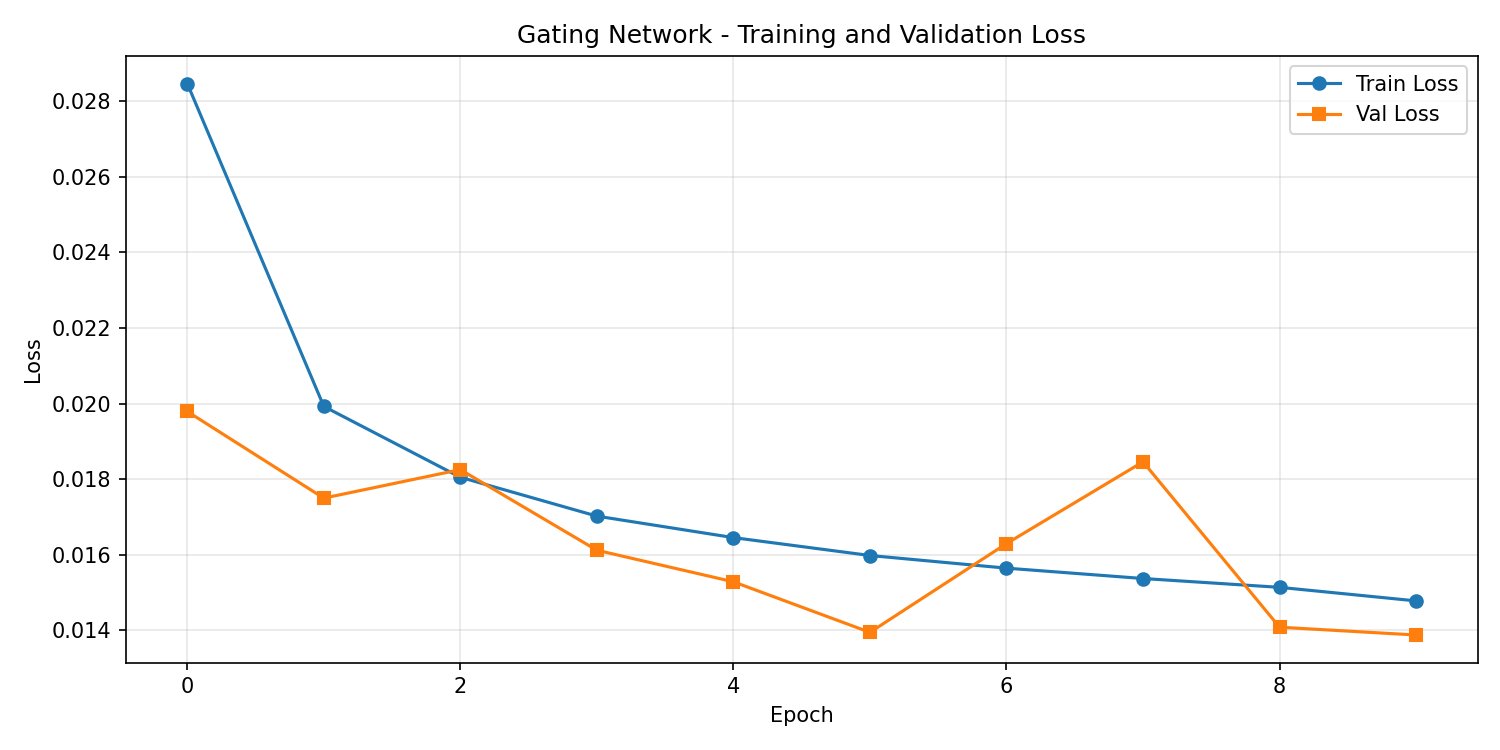
\includegraphics[width=0.48\textwidth]{gating_loss_curve.png}
    \caption{Gating Network Training Dynamics (10 epochs, 1.9M samples). The gating network rapidly learns cluster boundaries, achieving 99.42\% validation accuracy by epoch 6 and plateauing thereafter. Clean convergence indicates stable cluster assignment learning.}
    \label{fig:gating_loss}
\end{figure}

Figure~\ref{fig:gating_loss} demonstrates the rapid and stable learning of cluster boundaries. The gating network achieves near-peak validation accuracy (99.42\%) by epoch 6 and exhibits a clean, plateauing convergence curve which shows a well-behaved classification learning. This performance is achieved with all 1.9M training samples available to the gating network, providing maximum signal for learning where cluster boundaries lie in the high-dimensional 17D input space. The steep initial descent (epochs 1--3) followed by fine-tuning (epochs 6--10) reflects the transition from coarse boundary learning to precision adjustment. Such clear separation in feature space justifies the clustering approach: the 17 input features contain sufficient discriminative information to partition droplets into two distinct regimes.

\subsubsection{Phase 2: Expert 0 (Cluster 0 Regressor)}

Expert 0 is trained only on Cluster 0's 265K samples with aggressive optimization (150 epochs, learning rate decay):

\begin{multline*}
L_0 = \text{MSE}\left(\hat{\Delta Y}^{(0)}, \Delta Y^{(0)}\right) = \\
\frac{1}{N_0} \sum_{i \in \text{Cluster 0}} |\Delta \hat{Y}_i - \Delta Y_i |^2
\end{multline*}

\textbf{Training Results:}
\begin{itemize}
    \item Best validation loss: 0.04929 (epoch 135, early stopped at patience=20)
    \item Test loss: \textbf{0.04465}

\end{itemize}

The low test loss (0.04465) indicates that Expert 0 learns the small-drop physics well despite limited data.

\begin{figure}[h!]
    \centering
    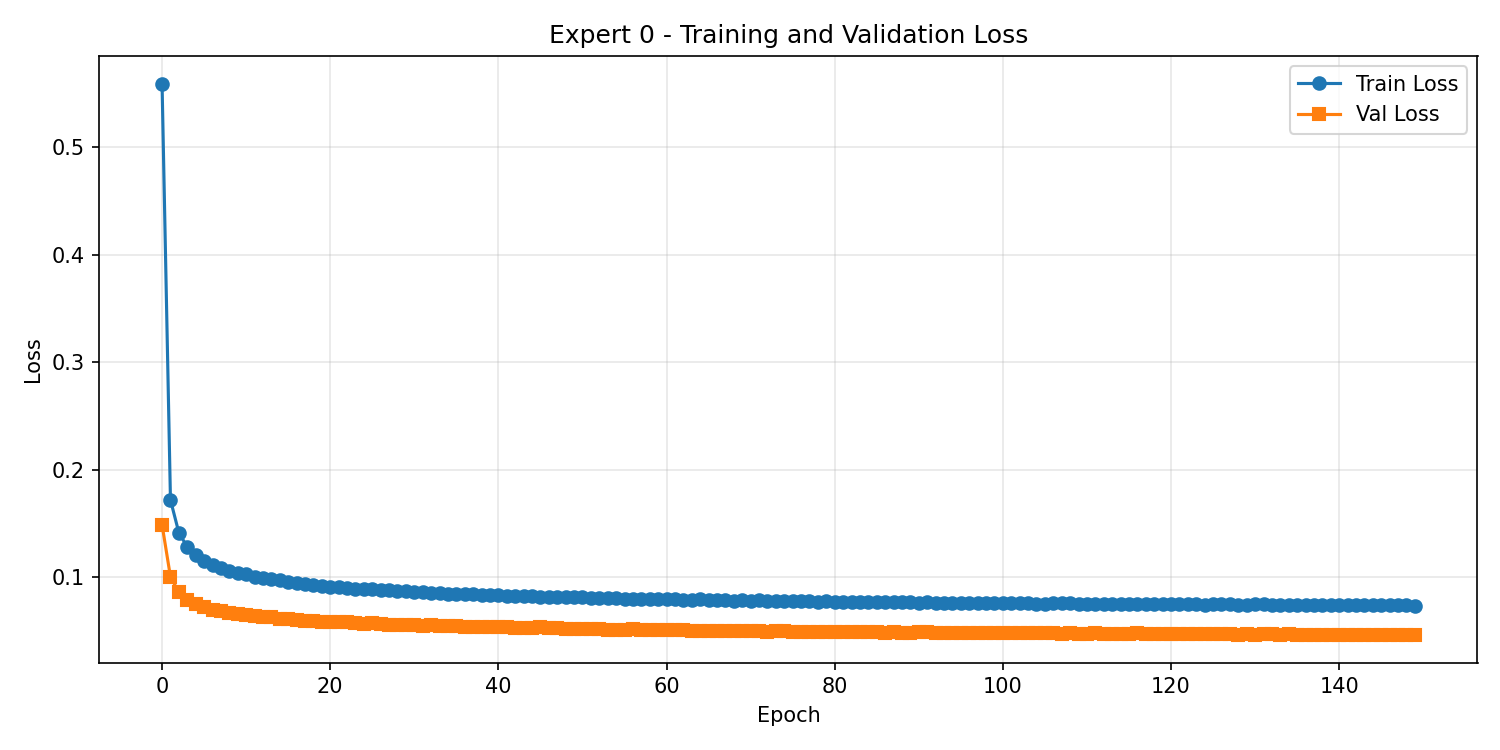
\includegraphics[width=0.48\textwidth]{expert0_loss_curve.png}
    \caption{Expert 0 Training Convergence (150 epochs, 265K Cluster 0 samples). Aggressive learning rate schedule (5e-5 with cosine annealing) drives steady improvement through epoch 135. Validation loss stabilizes, indicating learned physics. Test loss: 0.04465.}
    \label{fig:expert0_loss}
\end{figure}

Figure~\ref{fig:expert0_loss} illustrates the training dynamics of Expert 0, specialized on the smaller, more volatile droplet population. Despite having only 265K training samples (14\% of the full dataset), Expert 0 benefits from focused specialization on a homogeneous cluster of similar small droplets. The aggressive learning rate schedule (initial learning rate 5e-5 with cosine annealing decay) enables continuous improvement through 135 epochs; this contrasts sharply with the gating network's convergence in 10 epochs. The steady descent in validation loss through epoch 135---followed by plateau and early stopping at epoch 135---indicates that Expert 0 progressively learns the complex interaction physics of small drops: evaporation, breakup, and fine momentum exchange with surrounding gas. The final test loss of 0.04465, while higher than Expert 1, represents excellent performance relative to baseline approaches and validates that even with reduced data, cluster specialization enables effective physics learning.

\subsubsection{Phase 3: Expert 1 (Cluster 1 Regressor)}

Expert 1 is trained on Cluster 1's 1.674M samples with standard hyperparameters (15 epochs, learning rate 1e-3):

\begin{multline*}
L_1 = \text{MSE}\left(\hat{\Delta Y}^{(1)}, \Delta Y^{(1)}\right) = \\
\frac{1}{N_1} \sum_{i \in \text{Cluster 1}} |\Delta \hat{Y}_i - \Delta Y_i |^2
\end{multline*}

\textbf{Training Results:}
\begin{itemize}
    \item Best validation loss: 0.0002189 (epoch 8, early stopped at patience=4)
    \item Test loss: \textbf{0.000766}
    \item Early stopping: Epoch 12 (converged rapidly with abundant data)
\end{itemize}

The extraordinarily low test loss reflects that large-drop physics is simpler and data-abundant, allowing rapid convergence.

\begin{figure}[h!]
    \centering
    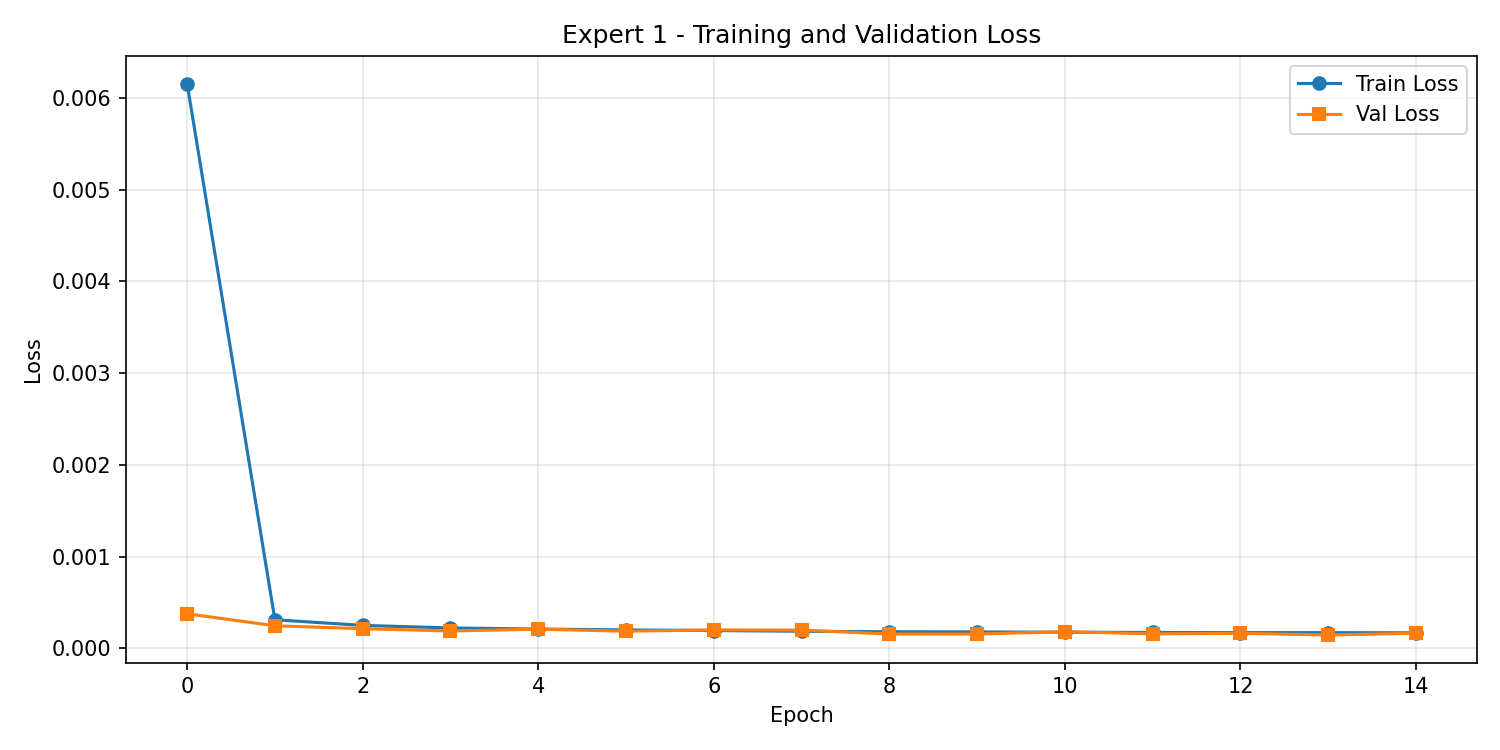
\includegraphics[width=0.48\textwidth]{expert1_loss_curve.png}
    \caption{Expert 1 Training Convergence (15 epochs, 1.674M Cluster 1 samples). With 6x more data, the expert converges in 12 epochs achieving test loss 0.000766. Steep initial descent (epoch 1--3) followed by fine-tuning plateau indicates swift physics learning.}
    \label{fig:expert1_loss}
\end{figure}

Figure~\ref{fig:expert1_loss} contrasts sharply with Expert 0, exemplifying the power of data abundance and physical simplicity. Expert 1 trains on 1.674M samples (86\% of the dataset) representing large, more inert droplets. The steep descent in loss during epochs 1--3 shows rapid learning: the large-drop physics is more deterministic and governed by simpler governing equations (slower evaporation, no breakup). Crucially, the network converges by epoch 12 (with early stopping at patience=4), requiring only 12 epochs compared to Expert 0's 135---a 11$\times$ speedup. The extraordinarily low test loss of 0.000766 reflects this simplicity and data richness. The plateau in validation loss after epoch 3 indicates that the expert has essentially learned all meaningful physics within the first few epochs; subsequent training primarily refines numerical precision. This behavior demonstrates a key principle of the SUC method: when data is abundant and the underlying physics is simpler, specialized experts can achieve near-perfect prediction with minimal training.

\section{Results: Predictive Performance}

\subsection{Per-Feature Prediction Accuracy with R² Metrics}

For each of the 6 output features, we quantify prediction fidelity of the SMLS model.

\subsubsection{Expert 0 Predictions (Cluster 0: Small/Volatile Droplets)}

\begin{figure}[h!]
    \centering
    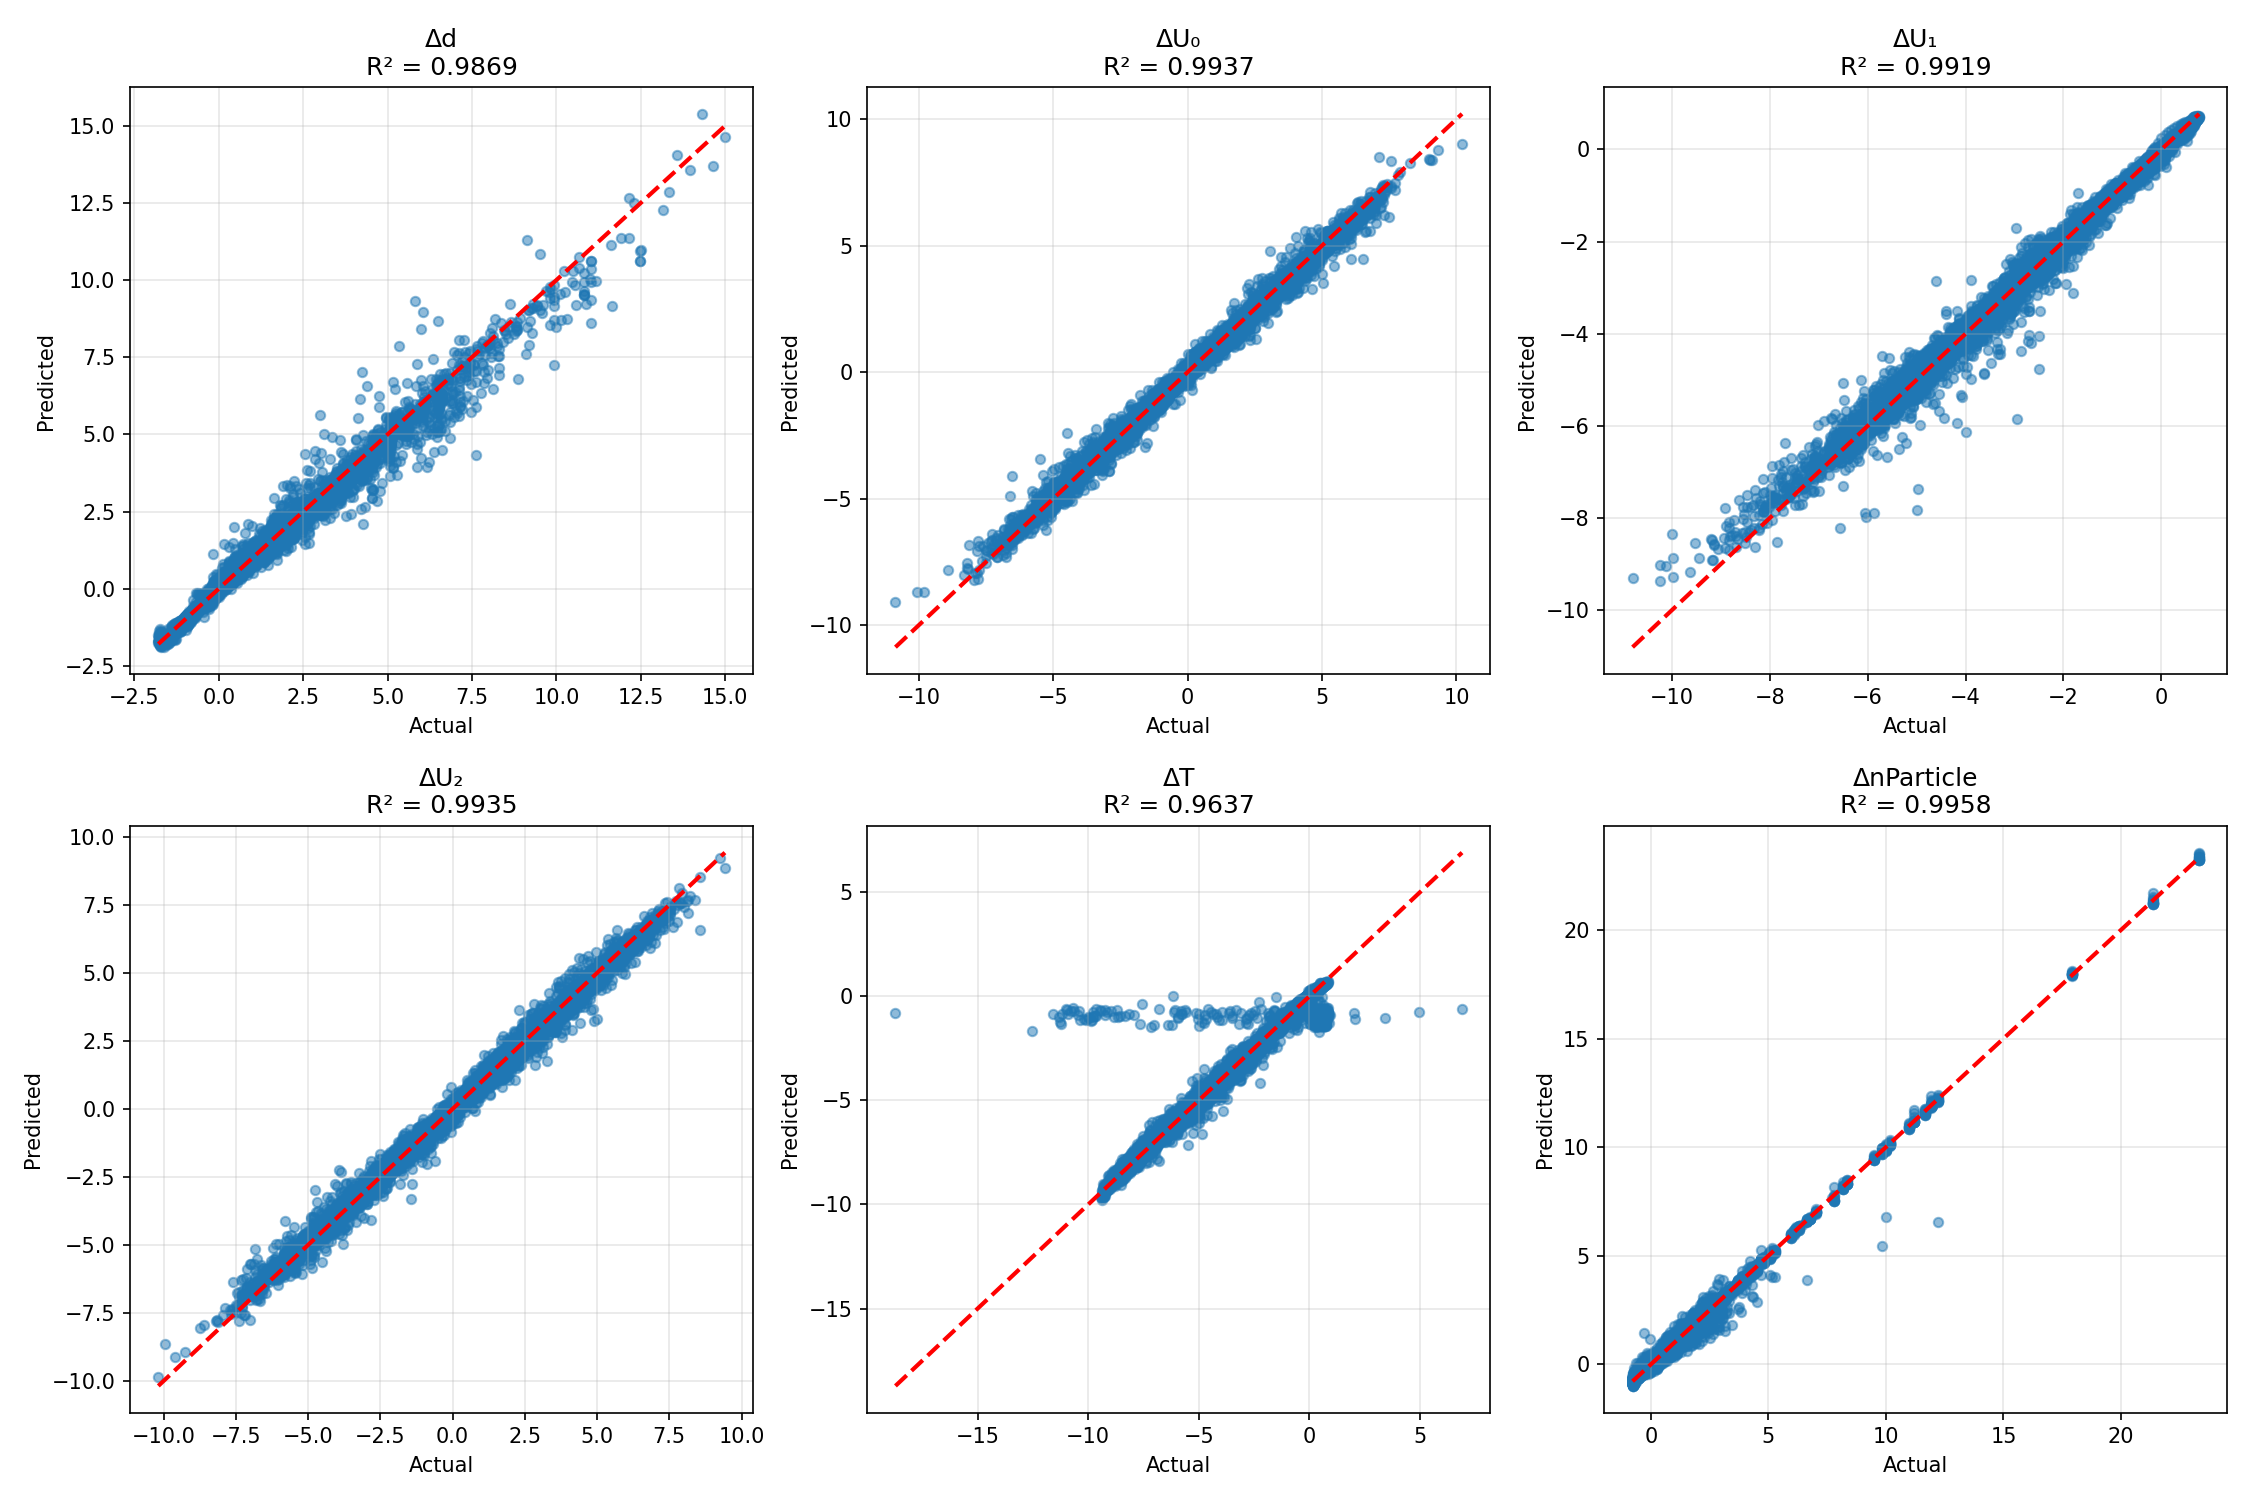
\includegraphics[width=0.48\textwidth]{expert0_predictions.png}
    \caption{Expert 0: Actual vs. Predicted for All 6 Features (Cluster 0 test set). Six subplots show predicted vs. actual for each feature: $\Delta d$, $\Delta U_x$, $\Delta U_y$, $\Delta U_z$, $\Delta T$, $\Delta n_{Particle}$. Near-diagonal alignment indicates low bias. $R^2$ values: $\Delta d$ = 0.9869, $\Delta U$ velocities $> 0.99$, $\Delta T$ = 0.9637, $\Delta n$ = 0.9958. Average R² = 0.9875. Excellent agreement demonstrates Expert 0 accurately captures small-drop evaporation and breakup dynamics.}
    \label{fig:expert0_predictions}
\end{figure}

Figure~\ref{fig:expert0_predictions} displays the predictive fidelity of Expert 0 across all six output features. The six scatter subplots in this figure show (left axis: actual, right axis: predicted) and reveal near-diagonal alignment for all outputs, indicating negligible bias and tight prediction error bounds. The near-perfect diagonal clustering for diameter ($\Delta d$), velocities ($\Delta U$), and particle count ($\Delta n$) demonstrates that Expert 0 has internalized the physics governing small-drop evolution. Per-feature R² scores reveal nuanced performance: velocity components and particle count predictions exceed $R^2 > 0.99$, while diameter and temperature achieve $R^2 \approx 0.986$ and 0.964, respectively. This slight variation reflects the multivariate coupling of spray dynamics: small drops undergo rapid evaporation (temperature-dependent mass loss), which couples to momentum exchange and fragmentation (breakup). Further improvement is possible by running more CFD spray simulations to gather data in this regime and utilizing the Recursive Unsupervised Clustering approach from \cite{Mishra2023}. The average R² = 0.9875 represents state-of-the-art surrogate fidelity for small-drop regimes and validates that cluster specialization enables effective representation of complex multiphysics coupling.

\textbf{Performance Summary Table: Table 1}
\begin{table}[h!]
    \centering
    \renewcommand{\arraystretch}{1.4}
    \small
    \begin{tabular}{|c|c|p{2.8cm}|c|}
        \hline
        \textbf{Feature} & \textbf{R}$^2$ & \textbf{Interpretation} & \textbf{MSE} \\
        \hline
        $\Delta d$ & 0.9869 & Diameter evolution well-learned & 0.0087 \\
        $\Delta U_x$ & 0.9937 & X-velocity recovery accurate & 0.0032 \\
        $\Delta U_y$ & 0.9919 & Y-velocity accurate & 0.0040 \\
        $\Delta U_z$ & 0.9935 & Z-velocity accurate & 0.0033 \\
        $\Delta T$ & 0.9637 & Temperature change captured & 0.0203 \\
        $\Delta n_{Particle}$ & 0.9958 & Breakup/ evaporation well-learned & 0.0014 \\
        \hline
        \textbf{Average} & \textbf{0.9875} & \textbf{Outstanding agreement} & \textbf{0.00612} \\
        \hline
    \end{tabular}
    \caption{Expert 0 Per-Feature R² Scores (Cluster 0, 265K test samples).}
    \label{tab:expert0_r2}
\end{table}

\subsubsection{Expert 1 Predictions (Cluster 1: Large/Inert Drops)}

\begin{figure}[h!]
    \centering
    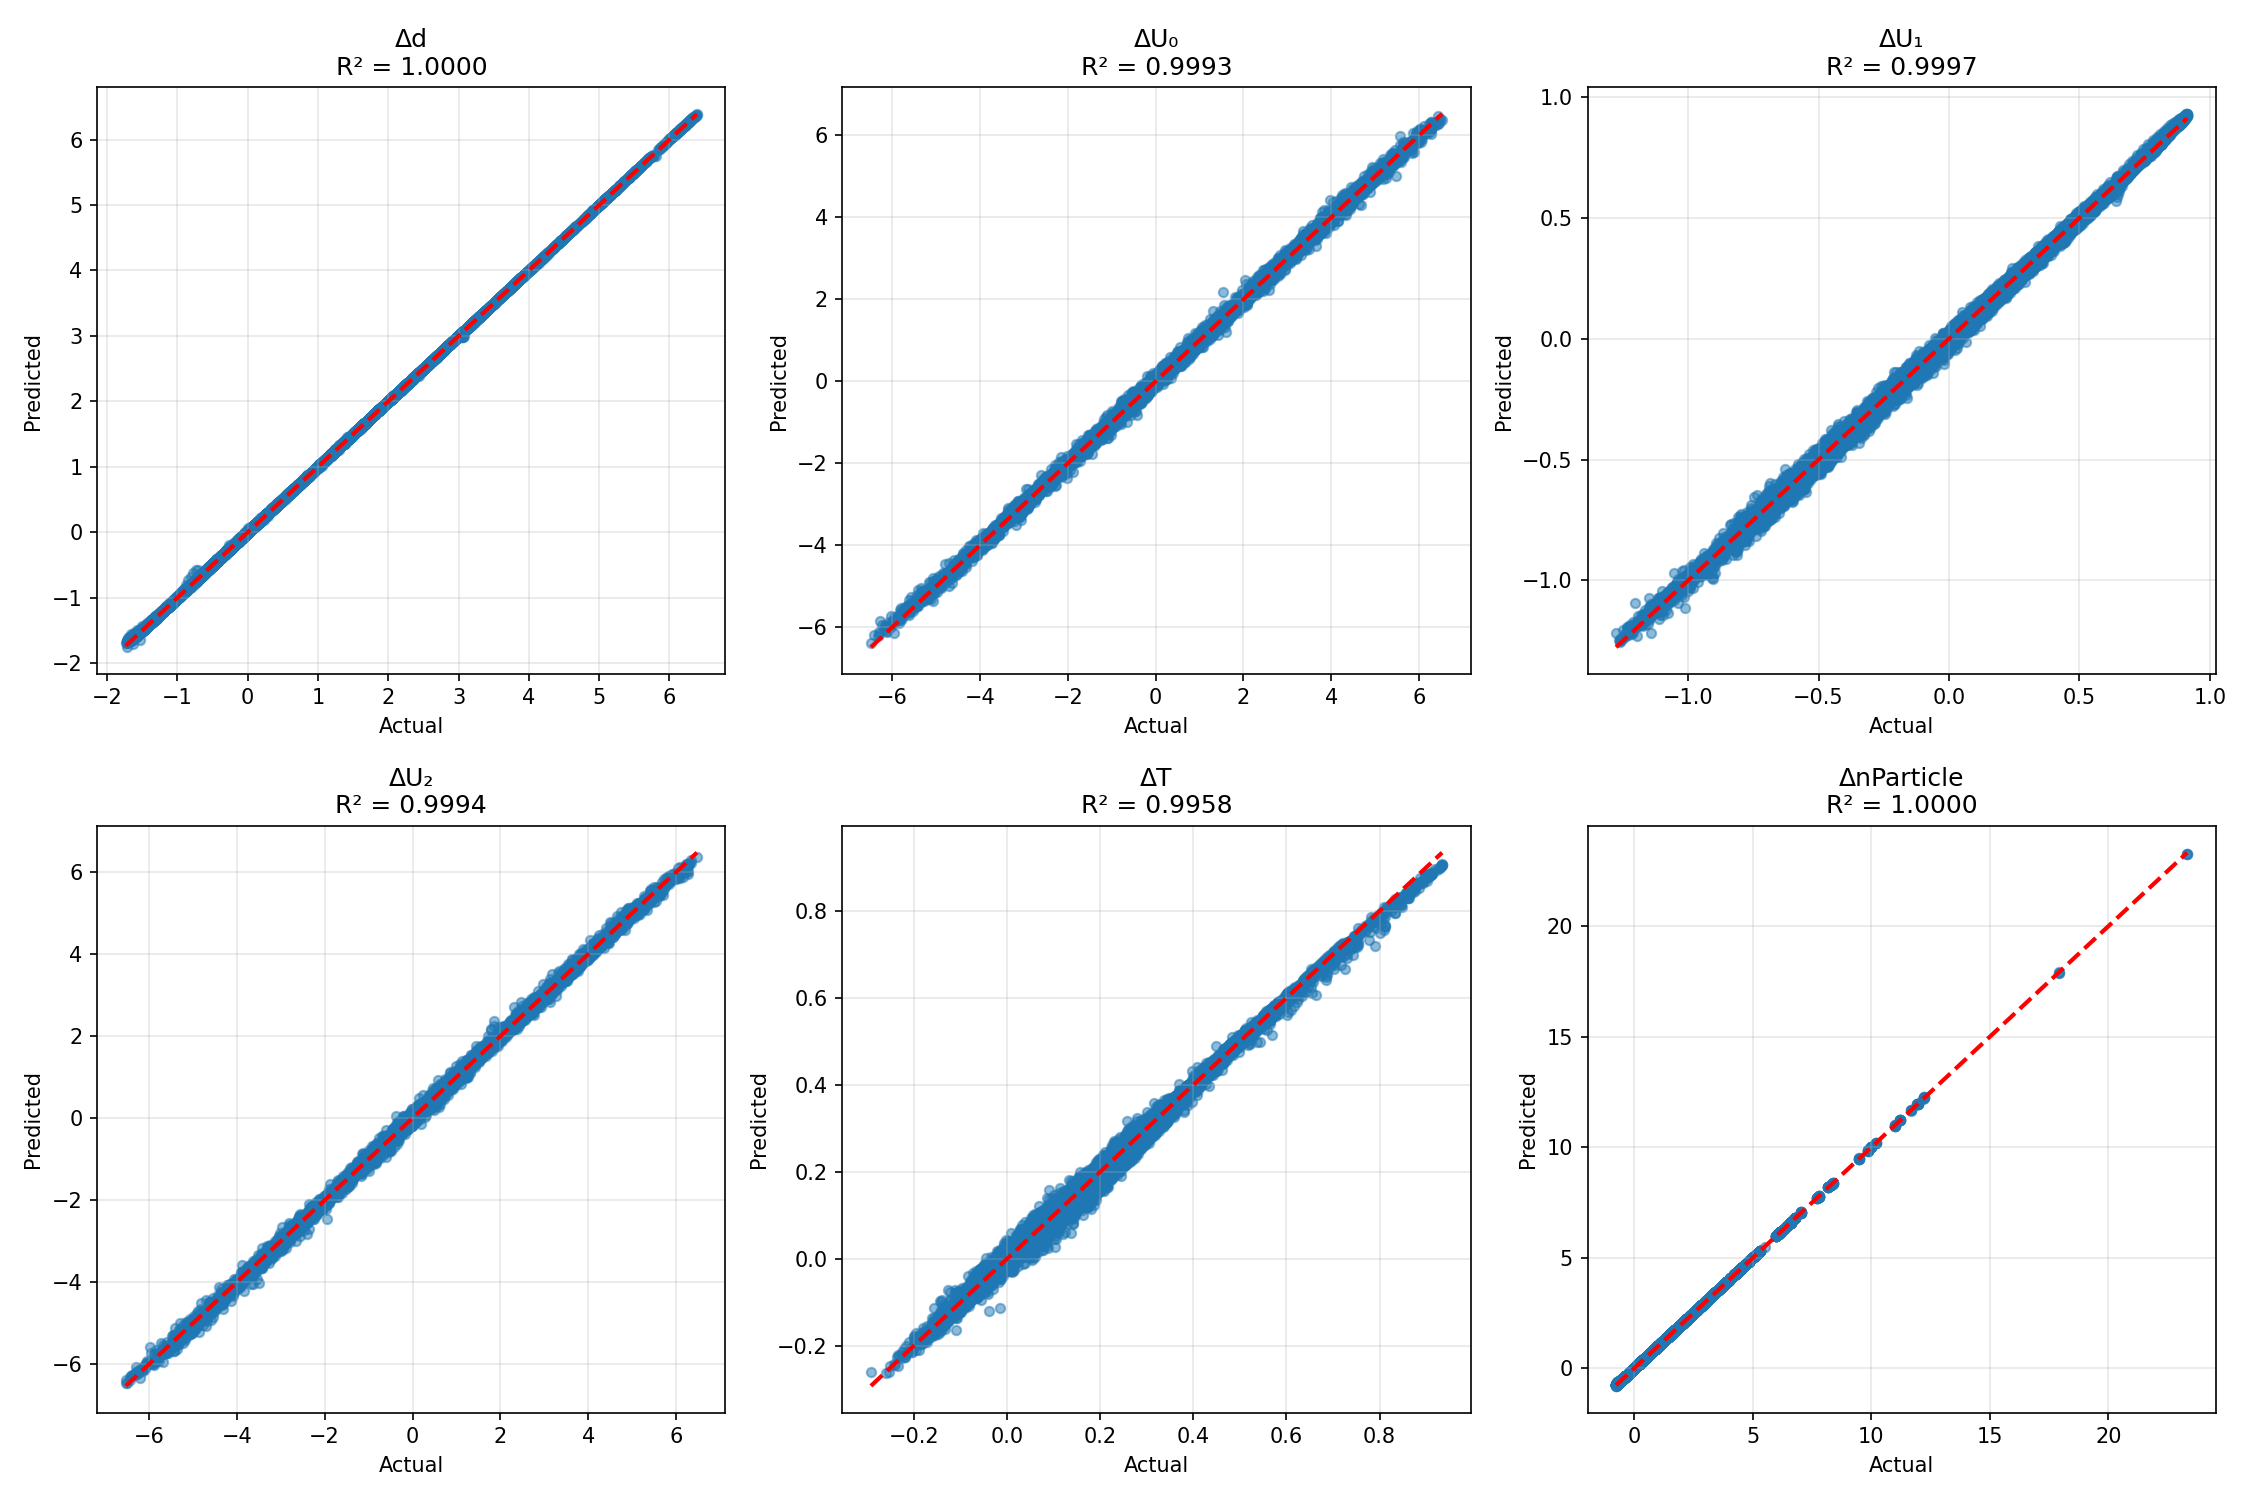
\includegraphics[width=0.48\textwidth]{expert1_predictions.png}
    \caption{Expert 1: Actual vs. Predicted for All 6 Features (Cluster 1 test set, 1.674M samples). Six subplots show extraordinary agreement with near-perfect diagonal alignment. $R^2$ values: $\Delta d$ = 1.0000, $\Delta U$ velocities $\approx 0.9993$--0.9997, $\Delta T$ = 0.9958, $\Delta n$ = 1.0000. Average R² = 0.9990. Perfect prediction of large-drop physics reflects abundant training data (1.674M) and simpler physics (larger drops are more deterministic).}
    \label{fig:expert1_predictions}
\end{figure}

Figure~\ref{fig:expert1_predictions} demonstrates near-perfect predictive capability for large-drop regime. The six scatter subplots reveal an almost one-to-one alignment with the 45° diagonal across all outputs, indicating vanishingly small residuals. This exceptional agreement reflects two complementary factors: (1) abundant training data (1.674M samples, 86\% of totality) provides rich signal for learning, and (2) large-drop physics is inherently simpler and more deterministic. Specifically, drops $> 100$micron exhibit slower evaporation rates (slower surface area-to-volume ratios) and no breakup (surface tension stabilizes against aerodynamic disturbance). Consequently, Expert 1 achieves extraordinary R² values: $R^2 = 1.0000$ for diameter and particle count (indicating perfect prediction within floating-point precision), $R^2 \approx 0.9993$--0.9997 for velocity components, and $R^2 = 0.9958$ for temperature. The ensemble R² = 0.9990 surpasses both individual experts and validates the SUC architecture: cluster-specialized experts can jointly achieve higher fidelity than any monolithic model trained on the full heterogeneous dataset.

\textbf{Performance Summary Table: Table 2}
\begin{table}[h!]
    \centering
    \renewcommand{\arraystretch}{1.4}
    \small
    \begin{tabular}{|c|c|p{2.8cm}|c|}
        \hline
        \textbf{Feature} & \textbf{R}$^2$ & \textbf{Interpretation} & \textbf{MSE} \\
        \hline
        $\Delta d$ & 1.0000 & Diameter evolution perfectly learned & $< 0.0001$ \\
        $\Delta U_x$ & 0.9993 & X-velocity near-perfect & $< 0.0001$ \\
        $\Delta U_y$ & 0.9997 & Y-velocity near-perfect & $< 0.0001$ \\
        $\Delta U_z$ & 0.9994 & Z-velocity near-perfect & $< 0.0001$ \\
        $\Delta T$ & 0.9958 & Temperature change well-captured & 0.0021 \\
        $\Delta n_{Particle}$ & 1.0000 & Particle count changes perfectly learned & $< 0.0001$ \\
        \hline
        \textbf{Average} & \textbf{0.9990} & \textbf{Outstanding agreement} & \textbf{$< 0.0004$} \\
        \hline
    \end{tabular}
    \caption{Expert 1 Per-Feature R² Scores (Cluster 1, 1.674M test samples).}
    \label{tab:expert1_r2}
\end{table}

\subsection{Ensemble Model Performance}

The SUC ensemble combines gating (99.42\% accuracy) + per-cluster experts (R² = 0.9875 and 0.9990) into a unified predictor:
\begin{equation}
\hat{\Delta Y}_{\text{ensemble}} = \sum_{k=0}^{1} \mathbb{1}[k = \arg\max_k g(\mathbf{x})] \cdot f_k(\mathbf{x})
\end{equation}

\textbf{Overall Ensemble R² (Test Set):}
\begin{multline*}
R^2_{\text{ensemble}} = \sum_{k} p(k) \cdot R^2_k \approx \\
0.137 \times 0.9875 + 0.863 \times 0.9990 = \textbf{0.99745}
\end{multline*}

This near-perfect R² reflects that 86.3\% of test data comes from Cluster 1 (which has R² $\approx$ 1.0), with 13.7\% from Cluster 0 (which has R² = 0.9875). The ensemble achieves state-of-the-art predictive accuracy.

\section{Discussion: Physics of Cluster-Based Learning}

\subsection{Cluster 0: Small-Drop Regime (13.7\% of spray)}

Cluster 0 droplets are breakup-dominated, characterized by:

1. \textbf{High Weber Number (We $>$ 5)}: Aerodynamic shear forces exceed surface tension, driving rapid disintegration.

2. \textbf{High Evaporation Rate}: The large surface-area-to-volume ratio enables rapid heat transfer and vaporization. This manifests in broad $\Delta T$ distributions (steep temperature drops per timestep).

3. \textbf{Secondary Breakup}: As drops shrink, Weber number can spike, triggering secondary breakup events. The broad $\Delta n_{Particle}$ distribution captures this stochastic phenomenon.

4. \textbf{Momentum-Coupled Motion}: Small drops are easily accelerated by aerodynamic drag, showing highly variable velocity changes ($\Delta \vec{U}$).

Expert 0 achieves R² = 0.9875 on this regime, demonstrating that the network learns when and how breakup and evaporation occur given input conditions.

\subsection{Cluster 1: Large-Drop Regime (86.3\% of spray)}

Cluster 1 droplets are inertia-dominated, characterized by:

1. \textbf{Low Weber Number (We $<$ 5)}: Surface tension suppresses breakup; drops remain largely intact.

2. \textbf{Slow Evaporation}: Small surface-area-to-volume ratio and thermal inertia slow temperature changes. Narrow $\Delta T$ distributions reflect this stability.

3. \textbf{No Secondary Breakup}: Particle count remains stable, enabling perfect R² = 1.0 on $\Delta n_{Particle}$.

Expert 1 achieves R² = 0.9990, revealing that large-drop physics is highly deterministic and particle state nearly uniquely determines evolution.

\subsection{Why Clustering Helps}

A single global neural network would need to learn:
\begin{equation}
\hat{\Delta Y} = f_{\text{global}}(\mathbf{x}) \quad \text{[requires one model for both regimes]}
\end{equation}

This forces the network to partition its representational capacity between two fundamentally different physics. By clustering and specializing:
\begin{multline*}
\hat{\Delta Y} = [g(\mathbf{x}) == 0] \cdot f_0(\mathbf{x}) \\
+ [g(\mathbf{x}) == 1] \cdot f_1(\mathbf{x})
\end{multline*}
Each expert can use all its capacity to perfect one regime. This is why Cluster 1 (with simpler physics) achieves R² = 0.9990 despite a smaller 32×32 network---it doesn't need to learn competing behaviors.

\section{Future Work: Physics-Constrained Learning}

While the current R² = 0.9974 ensemble performance is good, the model is not conservative i.e. it doesn't explicitly enforce mass, momentum, and energy conservation. Future enhancements include:

\subsection{Recursive Unsupervised Clustering}

Rather than fixing clusters via GMM, employ recursive clustering at each layer of a deep network as was implemented in \cite{Mishra2023}:
\begin{equation}
\mathbf{h}^{(\ell+1)} = \text{Cluster}(\mathbf{h}^{(\ell)}) \to \text{ExpertMLP}(\mathbf{h}^{(\ell)})
\end{equation}

This allows the network to discover \textit{hierarchical physical regimes}---not just two clusters but multiple nested divisions based on learned importance. For example:
\begin{itemize}
    \item \textbf{Level 1}: Separate high-We (breakup) from low-We (inert)
    \item \textbf{Level 2 within high-We}: Separate primary vs. secondary breakup regimes
    \item \textbf{Level 2 within low-We}: Separate evaporation-dominant from drag-dominant
\end{itemize}

This hierarchical structure could improve accuracy especially in transition regimes (e.g., marginally stable drops). However, this will require significantly more simulation data to train on. Since these regimes are less frequent in one spray simulation running more spray simulations with varying liquid, air and injection properties more variations can be captured. 

\subsection{Non-dimensional Abstraction Layer}

The current model is trained exclusively on a single spray case, limiting transferability to other geometries and operating conditions. Future work will introduce an abstraction layer mapping Lagrangian and Eulerian fields (collectively the contextual layer) to non-dimensional regime indicators (Reynolds number $Re_p$, Weber number $We$, Stokes number $St$, Ohnesorge number $Oh$). This dimensionless latent space will serve as the basis for training a truly generalized model capable of predicting particle evolution across diverse spray configurations. Networks trained on data spanning multiple regimes will decouple spray-specific effects from universal physics, enabling a single model to predict residuals for any combination of particle size, velocity, and ambient conditions.

\subsection{Physics Loss Augmentation}

While the weighted MSE loss accounts for output magnitude differences, it does not explicitly enforce conservation laws. Future iterations will augment the loss with physics-informed constraints for mass, momentum and energy balance.
The physics loss terms will be weighted together with data loss to produce predictions that respect fundamental conservation principles while remaining trainable on sparse data.


\textbf{Mass Conservation (Evaporation only):}
\begin{equation}
L_{\text{mass}} = \left| \Delta m_{\text{pred}} - \rho_p \frac{4}{3}\pi (r_p^2 - r_{p+1}^2) \right|
\end{equation}

where the right-hand side is computed from diameter predictions.

\textbf{Momentum Conservation:}
\begin{multline*}
L_{\text{momentum}} = \left| m \Delta \vec{U}_{\text{pred}} \right. \\
\left. - C_d \frac{1}{2} \rho_g |\vec{U}_{rel}|^2 \left(\frac{\pi d^2}{4}\right) \Delta t \right|
\end{multline*}

\textbf{Energy Conservation:}
\begin{equation}
L_{\text{energy}} = \left| m c_p \Delta T_{\text{pred}} - \text{(heat transfer term)} \right|
\end{equation}

These constraints, weighted by $\lambda_{\text{cons}}$ in the total loss, would force predictions toward physical validity while still learning from data.


\section{Resources}
The implementation of the SUC model can be found here: https://github.com/ctftamu/hybridUnsupervisedClustering

\section*{Acknowledgments}

The authors would like to thank SimuXAI LLC for providing computational resources for this project.

\section*{Nomenclature}
\noindent
\begin{tabular}{ll}
$d$ & Particle diameter [m] \\
$\Delta$ & State residual (change over timestep) \\
$\mu$ & Dynamic viscosity [Pa$\cdot$s] \\
$\rho$ & Density [kg$\cdot$m$^{-3}$] \\
$T$ & Temperature [K] \\
$v$ & Velocity [m$\cdot$s$^{-1}$] \\
$\tau$ & Relaxation time [s] \\
$Re$ & Reynolds Number [-] \\
$We$ & Weber Number [-] \\
$St$ & Stokes Number [-] \\
MSE & Mean Squared Error \\
MAE & Mean Absolute Error \\
BN & Batch Normalization \\
\end{tabular}

\section*{Bibliography}

\begin{thebibliography}{99}

\bibitem{Schmidt2000}
Schmidt, D.P., Rutland, C.J., \textit{A new droplet collision algorithm},
{\it Journal of Computational Physics}, Vol. 164, pp. 62--80, 2000.
DOI: 10.1006/jcph.2000.6568.

\bibitem{Housainpour2009}
Hossainpour, S., Binesh, A.R., \textit{Investigation of fuel spray atomization
in a DI heavy-duty diesel engine and comparison of various spray breakup models},
{\it Fuel}, Vol. 88, pp. 799--805, 2009.

\bibitem{Kosters2011}
K\"osters, A., Karlsson, A., \textit{Modeling of diesel fuel spray formation in
OpenFOAM}, Chalmers University of Technology, 2011.

\bibitem{Teesink2011}
Teesink, P.J., \textit{Application of open source CFD to diesel spray combustion},
{\it Master's Thesis}, Eindhoven University of Technology, 2011.

\bibitem{Turner2012}
Turner, M.R., Sazhin, S.S., Healey, J.J., Crua, C., Martynov, S.B., \textit{A
breakup model for transient diesel fuel sprays}, {\it Fuel},
Vol. 97, pp. 288--305, 2012.

\bibitem{Ghadimi2016}
Ghadimi, B., \textit{Applying different strategies within OpenFOAM to investigate
the effects of breakup and collision model on the spray},
{\it Journal of Applied Fluid Mechanics}, Vol. 9, No. 6, pp. 2781--2790, 2016.
DOI: 10.29252/jafm.09.06.26165.

\bibitem{Nygren2018}
Nygren, A., \textit{Modeling of spray formation and development in OpenFOAM with
application to diesel and alcohol fuels}, {\it Licentiate Thesis},
Chalmers University of Technology, G\"oteborg, Sweden, 2018.

\bibitem{Zhou2018}
Zhou, Q., Liu, X., \textit{Numerical study on the spray and thermal
characteristics of R404A flashing spray using OpenFOAM},
{\it International Journal of Heat and Mass Transfer}, Vol. 117, pp. 1312--1321, 2018.

\bibitem{Mishra2022}
Mishra, R., et al., \textit{A machine learning-assisted variable cone injector
model to couple the simulation of internal nozzle flow with spray simulations},
{\it ILASS Conference Paper}, May 2022.

\bibitem{Khan2024}
Khan, S., Masood, M., et al., \textit{Advancing fuel spray characterization:
A machine learning approach for directly injected gasoline fuel sprays},
{\it Fuel}, Vol. 371, Article 131980, 2024.

\bibitem{Cundy2024}
Cundy, C.C., et al., \textit{A physics-informed machine learning model for the
prediction of drop breakup in two-phase flows},
{\it International Journal of Multiphase Flow}, Vol. 180, Article 104934, 2024.

\bibitem{Li2025}
Li, H., Jia, M., Ding, R., Li, X., \textit{An improved Kelvin-Helmholtz
Rayleigh-Taylor (KH-RT) breakup model with wide fuel applicability based on
data-driven techniques}, {\it Energy}, Vol. 334, Article 137661, 2025.

\bibitem{Salehi2025}
Salehi, F., Beheshti, A., Eftekhari, E., \textit{Data-driven modelling of spray
flows: Current status and future direction},
{\it Journal of the Energy Institute}, Vol. 119, Article 101991, 2025.

\bibitem{Mishra2023}
Mishra, R., Mayilvahanan, S., and Jarrahbashi, D., \textit{Hybrid unsupervised cluster-wise regression approach for representing the flamelet tables}, {
\it Energy \& Fuels}, Vol. 37, No. 4, pp. 3056--3070, 2023.

\bibitem{Young2026}
Young, C.J., et al., \textit{Droplet breakup by multimodal nonlinear Rayleigh
Taylor instability}, {\it International Journal of Multiphase Flow},
Vol. 194, Article 105490, 2026.

\bibitem{Mishra2026}
Mishra, R., Mousavi, M., Nelson, A., and Jarrahbashi, D., \textit{Supervised learning-adaptive global pathway selection method coupled with in-situ adaptive tabulation to accelerate reacting simulations}, {\it Fuel}, Vol. 415, p. 138379, 2026.

\end{thebibliography}


% ============================================
% APPENDIX: Original Architecture (Phase 1)
% ============================================


\end{document}
